\chapter{実験}
\label{chap:ex}

%----------------------------------------------
\section{まえがき}
%----------------------------------------------
前章で提案したDNNに基づくパーミュテーション解決法の有効性を確認するために,人工的に作成したデータと実際の音声及び音楽信号を用意し,提案パーミュテーション解決法を適用してその性能を評価した.
\ref{sec:ex_condition}節では,本実験における条件を詳細に示し,\ref{sec:ex_res}節では提案手法のパーミュテーション解決性能を示している.
\ref{sec:matome}節で本章のまとめを述べる.
%----------------------------------------------
\section{実験条件}
\label{sec:ex_condition}
%----------------------------------------------
% \begin{table}[t]
% \begin{center}
%  \caption{Experimental conditions}
%  \label{table:ex}
%   \begin{tabular}{clll}\hline \hline
%    Window function in STFT & Hamming window  \\ \hline
%    Window length in STFT & 512~ms  \\ \hline
%    Shift length in STFT & 128~ms \\ \hline
%    Paramaters in Adam optimizer & \begin{tabular}{c}
%    \begin{flushleft}Learning rate = $0.001$\end{flushleft}\\
%    \begin{flushleft}$\beta = 0.9$\end{flushleft}
%    \end{tabular}  \\ \hline 
%    Reverberation time & $T_{60} = 470$~ms\\ \hline
%    Source direction of training data & $(\theta_1, \theta_2)=(60^\circ, 120^\circ)$\\ \hline
%    Source direction of test data & \begin{tabular}{c}
%    \begin{flushleft}(\theta_1, \theta_2)=(60^\circ, 120^\circ)\end{flushleft}\\ 
%    \begin{flushleft}(\theta_1, \theta_2)=(60^\circ, 100^\circ)\end{flushleft}\\ 
%    \begin{flushleft}(\theta_1, \theta_2)=(70^\circ, 110^\circ)\end{flushleft}
%    \end{tabular}\\ \hline \hline
%   \end{tabular}
%  \end{center}
% \end{table}
本実験では,提案する深層パーミュテーション解決法において,どの程度各周波数成分の正しい並び替えができるかを実験的に確認した.
本実験では,まず最初に基礎実験として,音響信号ではなく人工的に作成した2次元の行列を用いた性能評価を実施した.
人工的に作成した行列を2つ用意してパーミュテーション問題を模擬することで推定信号を生成し,これらを提案手法に入力してどの程度パーミュテーション問題が解決されるかを評価した.
この基礎実験における詳細な実験条件については\ref{sec:ex_condition_matrix}項に示す.
次に,実際の音響信号(音声及び音楽信号)の振幅スペクトログラムに対する性能評価も実施した.
基礎実験の場合と同様にパーミュテーション問題を模擬し,提案手法に入力して性能を評価した.
実際の音響信号を用いた実験の詳細な実験条件については,\ref{sec:ex_condition_audio}項に示す.
%----------------------------------------------
\subsection{人工データを用いた基礎実験の条件}
\label{sec:ex_condition_matrix}
%----------------------------------------------
基礎実験ではまず,パーミュテーション問題の生じていない(完全に解決された状態の)分離信号$(\bm{Z}_1, \bm{Z}_2)$として,Figs.~\ref{fig:01mat_spec}--\ref{fig:stripe_spec}に示す3種類の2次元行列のペアを用いた.
これらはいずれもサイズが$I=J=100$であり,それぞれ下記の構造を持っている.
\begin{itemize}
  \item 全成分が0の$\bm{Z}_1$と全成分が1の$\bm{Z}_2$(Fig.~\ref{fig:01mat_spec})
  \item 25列毎に0と1が入れ替わる$\bm{Z}_1$及び$\bm{Z}_2$(Fig.~\ref{fig:25stripe_spec})
  \item 1列毎に0と1が入れ替わる$\bm{Z}_1$及び$\bm{Z}_2$(Fig.~\ref{fig:stripe_spec})
\end{itemize}
次に,分離信号$(\bm{Z}_1, \bm{Z}_2)$の各行ベクトルを音源間でランダムに入れ替えることでパーミュテーション問題を模擬し,パーミュテーション問題が生じている推定信号$(\bm{Y}_1, \bm{Y}_2)$を生成した.
このとき,FDICAで一般的に生じるような(Fig.~\ref{fig:permu}のような)1行単位でランダムに入れ替わるパーミュテーション問題だけでなく,
Fig.~\ref{fig:bp}のような複数行のブロック単位でまとまって入れ替わるブロックパーミュテーション問題を模擬した推定信号$(\bm{Y}_1, \bm{Y}_2)$も生成した.
ブロックパーミュテーション問題を模擬する際の各ブロックの行数は,Fig.~\ref{fig:ex_block}に示すように$\gamma$行と定義し,これを$\gamma=1, 2, 4, 8$の4種類として実験した($\gamma=1$は通常の1行毎のパーミュテーション問題に対応).
従って,3種類の分離信号のペア$(\bm{Z}_1, \bm{Z}_2)$と4種類のブロック単位の合計12種類の実験条件を用意した.

本基礎実験では,前述の12種類の各実験条件のそれぞれに対して専用の深層パーミュテーション解決法(DNN)を学習した.
従って,各DNNを学習する際に用いる学習データは,各実験条件に従う推定信号$(\bm{Y}_1, \bm{Y}_2)$(入力)及び分離信号$(\bm{Z}_1, \bm{Z}_2)$(ラベル)であり,
入力はパーミュテーション問題を模擬するランダムな入れ替えを300パターン(重複無し)生成することで学習データを構築した.
この300パターンの推定信号$(\bm{Y}_1, \bm{Y}_2)$に対するラベルはパーミュテーション問題が解決された信号であるため,常に同じ分離信号$(\bm{Z}_1, \bm{Z}_2)$となる.
また,性能評価に用いる検証データとテストデータは同一とし,学習データの300パターンには含まれていないランダムな入れ替えでパーミュテーション問題を模擬した1パターンの推定信号$(\bm{Y}_1, \bm{Y}_2)$を用いた.
DNNの最適化法にはAdam~\cite{adam}を用い,Adamのハイパーパラメータはそれぞれ$\varepsilon=1.0\times10^{-8}$,$\beta_1 = 0.9$,$\beta_2 = 0.999$,及び学習率$\eta=0.001$に設定した.
その他の学習パラメータについては,バッチサイズを8,エポック数を1000として誤差逆伝播による学習を行った.

深層パーミュテーション解決法の性能を評価するための客観評価尺度には,正しく並び替えを行うことができた行の割合,即ち検証データに対する正答率を用いる.


%%%%%%%%%%%%%%%%%%%%%%%%%%%%
\begin{figure}[t]
  \begin{center}
      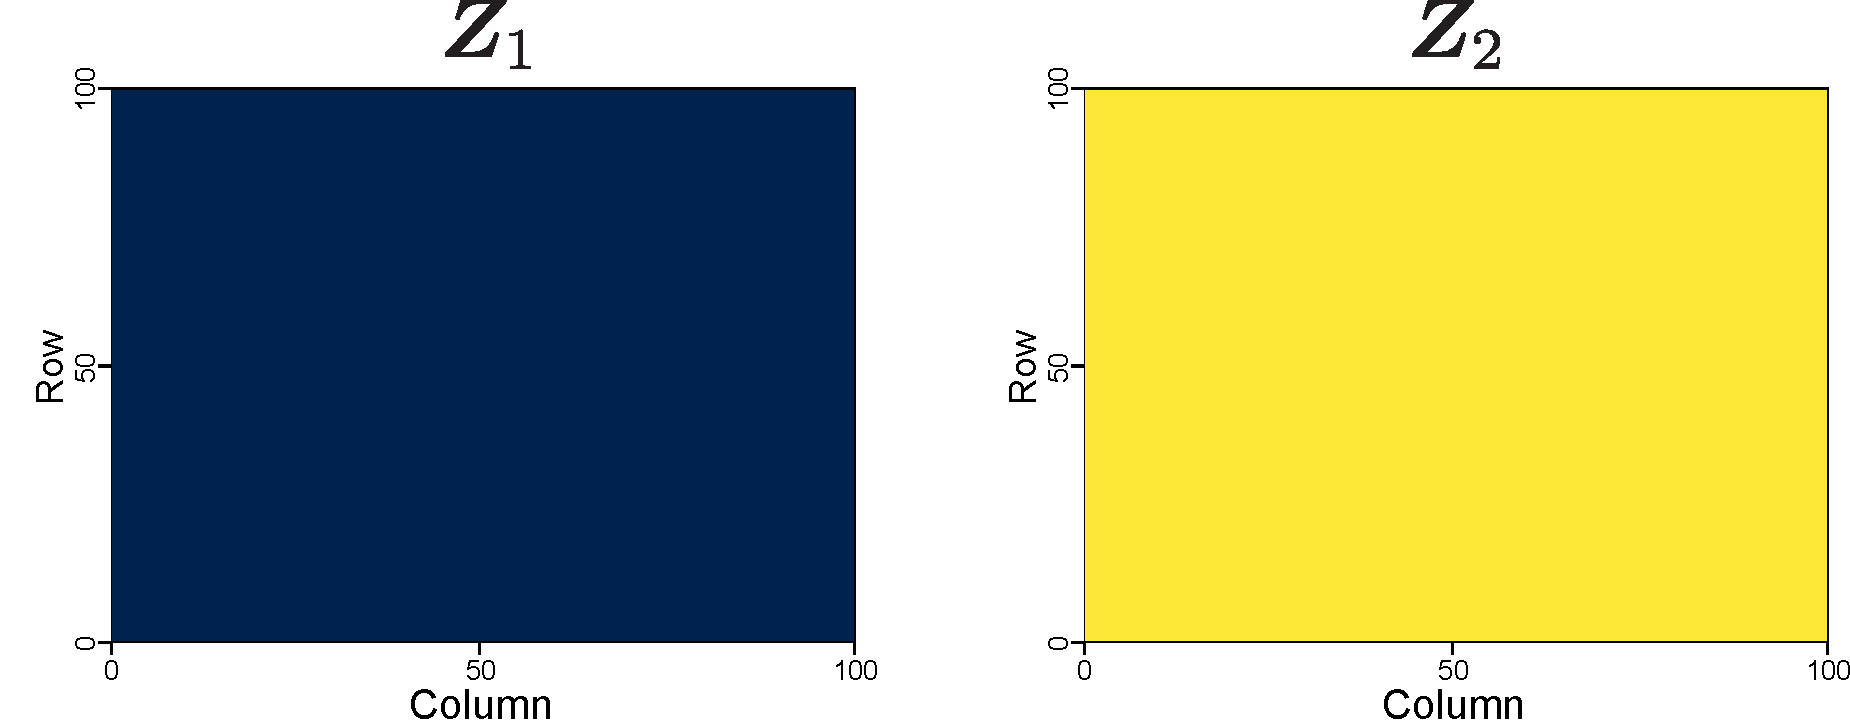
\includegraphics[width=0.95\columnwidth]{figures/origi_spec/01mat.pdf}
  \end{center}
\caption{Artificial source matrices $(\bm{Z}_1, \bm{Z}_2)$ with only zero or one elements.}
\label{fig:01mat_spec}
\end{figure}
%%%%%%%%%%%%%%%%%%%%%%%%%%%%

%%%%%%%%%%%%%%%%%%%%%%%%%%%%
\begin{figure}[t]
  \begin{center}
      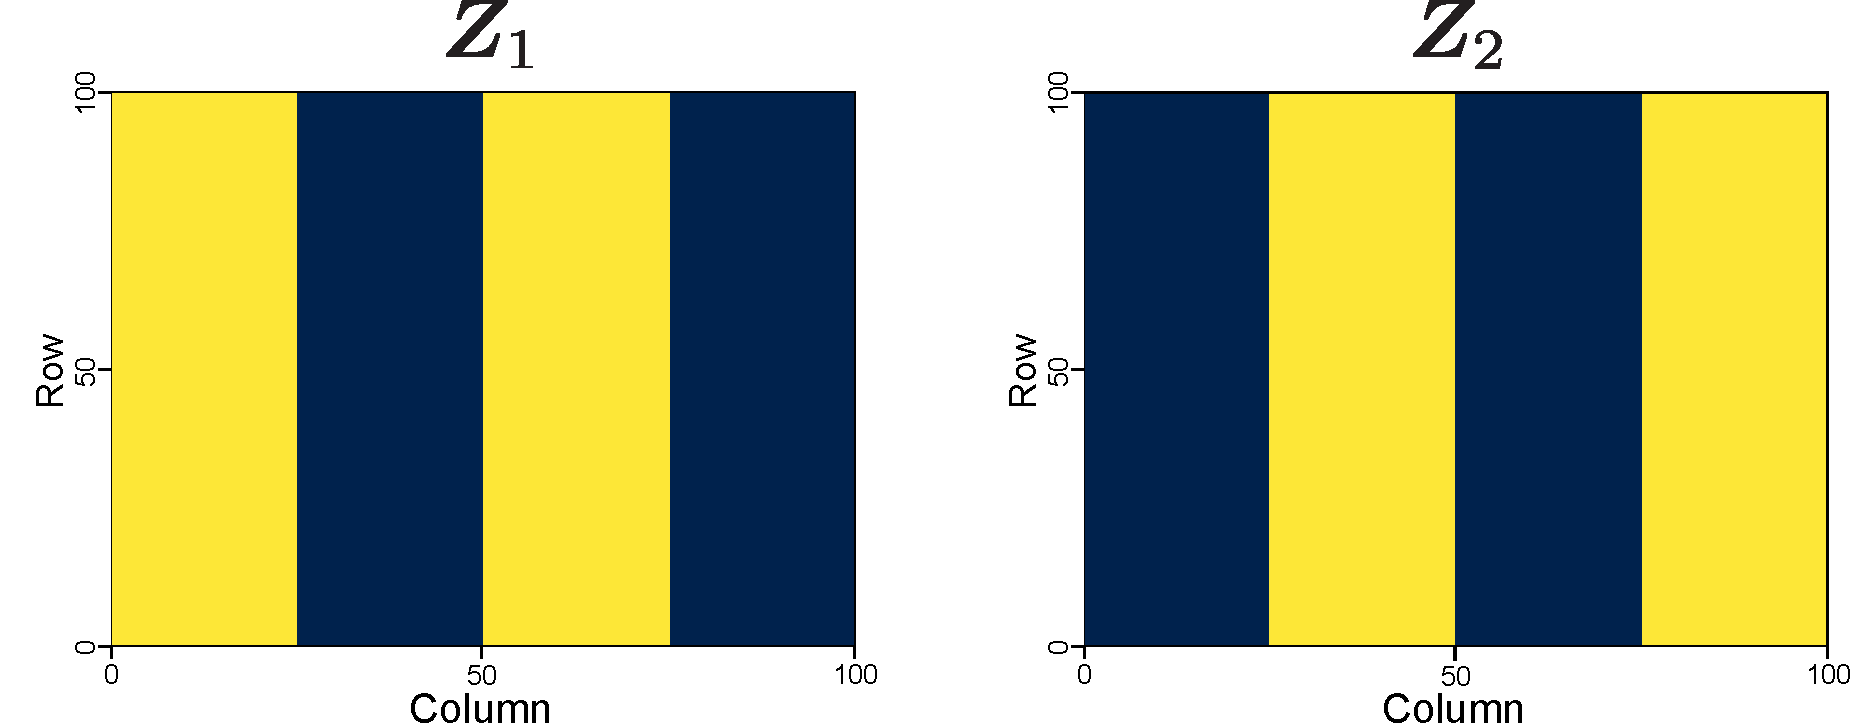
\includegraphics[width=0.95\columnwidth]{figures/origi_spec/25stripe.pdf}
  \end{center}
\caption{Artificial source matrices $(\bm{Z}_1, \bm{Z}_2)$ with zero and one elements swapping every 25 columns.}
\label{fig:25stripe_spec}
\end{figure}
%%%%%%%%%%%%%%%%%%%%%%%%%%%%

%%%%%%%%%%%%%%%%%%%%%%%%%%%%
\begin{figure}[t]
  \begin{center}
      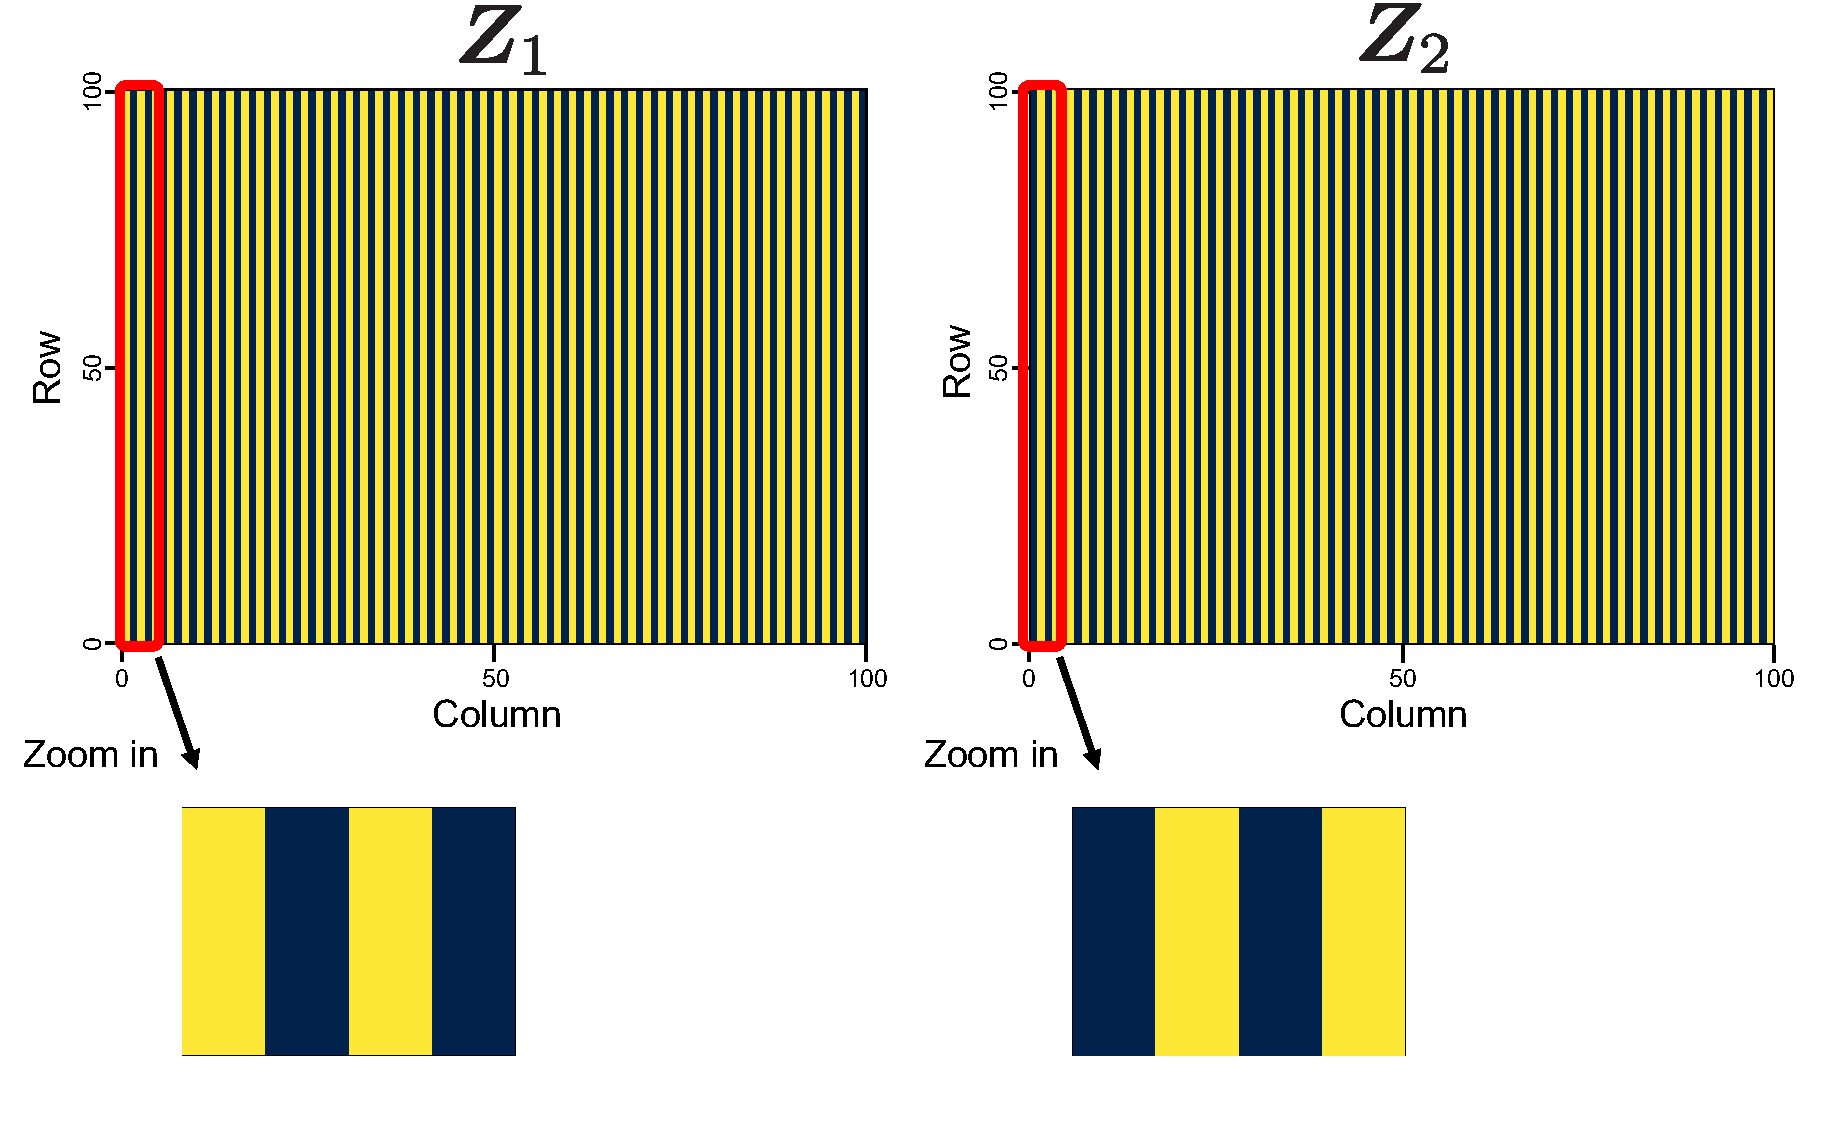
\includegraphics[width=0.95\columnwidth]{figures/origi_spec/stripe.pdf}
  \end{center}
\caption{Artificial source matrices $(\bm{Z}_1, \bm{Z}_2)$ with zero and one elements swapping every columns.}
\label{fig:stripe_spec}
\end{figure}
%%%%%%%%%%%%%%%%%%%%%%%%%%%%

%%%%%%%%%%%%%%%%%%%%%%%%%%%%
\begin{figure}[t]
    \begin{center}
        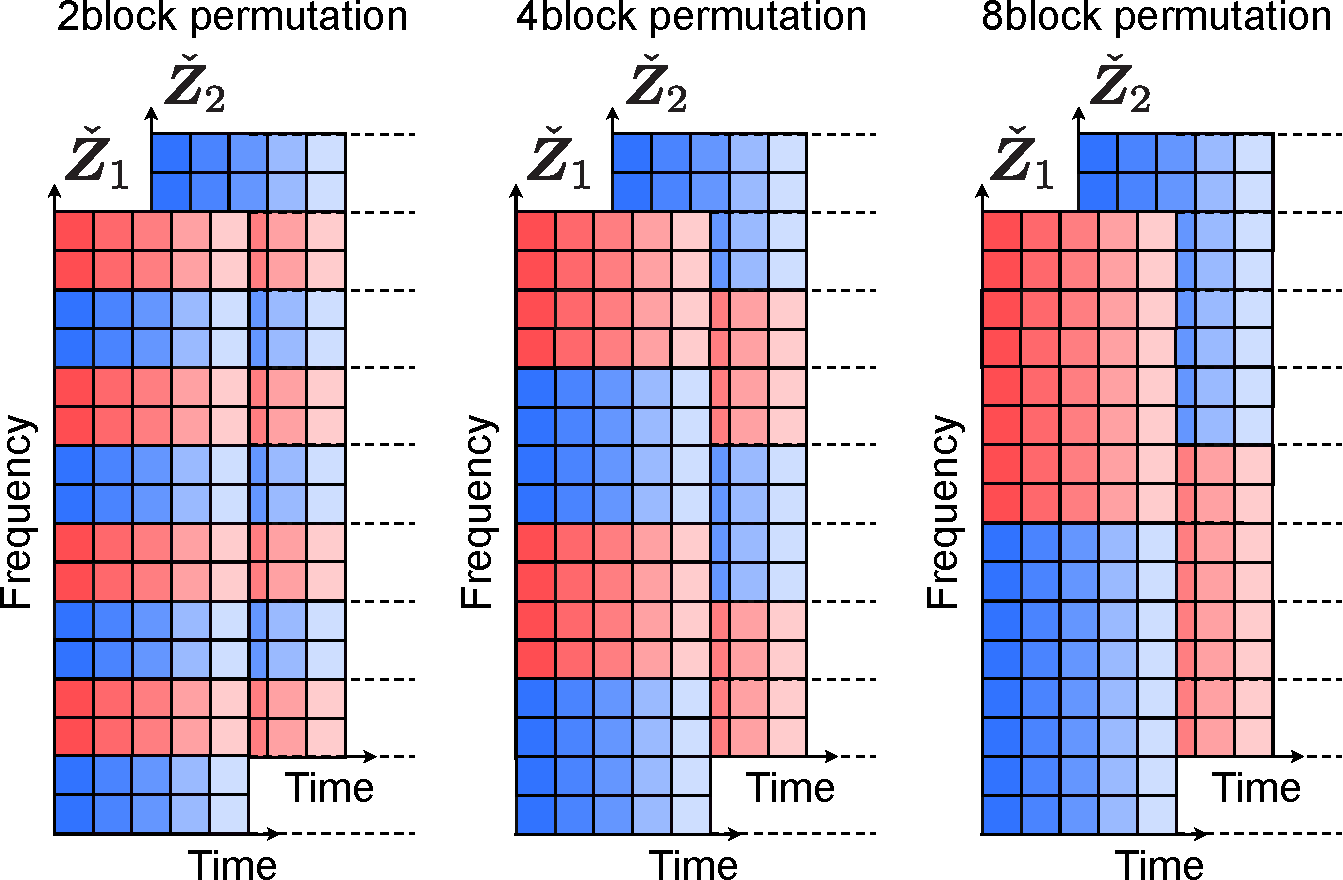
\includegraphics[width=0.70\columnwidth]{figures/experiment_block_matrix.pdf}
    \end{center}
	\caption{Simulation of block permutation problems, where $\gamma$ is row size of each block.}
	\label{fig:ex_block}
\end{figure}
%%%%%%%%%%%%%%%%%%%%%%%%%%%%

\clearpage
%----------------------------------------------
\subsection{実際の音響信号を用いた実験の条件}
\label{sec:ex_condition_audio}
%----------------------------------------------

%----------------------------------------------

%%%%%%%%%%%%%%%%%%%%%%%%%%%%
\begin{table}[t]
  \begin{center}
   \caption{Speech sources obtained from SiSEC2011}
   \label{table:wav}
    \begin{tabular}{clll}\hline \hline
     Signal type  & Data name &Length~[s]  \\ \hline
     Speech  & dev3\_female4\_src\_2 & 10.0  \\ \hline
     Speech  & dev2\_male4\_src\_2 &  10.0 \\ \hline
     \hline
    \end{tabular}
   \end{center}
\end{table}
%%%%%%%%%%%%%%%%%%%%%%%%%%%%

%%%%%%%%%%%%%%%%%%%%%%%%%%%%
\begin{table}[t]
  \begin{center}
   \caption{Music instrument sources obtained from SiSEC2011}
   \label{table:instrument}
    \begin{tabular}{clll}\hline \hline
     Signal type  & Data name &Length~[s]  \\ \hline
     Piano   & dev2\_nodrums\_liverec\_250ms\_src\_3 & 11.0\\ \hline
     Drums   & dev2\_wdrums\_liverec\_250ms\_src\_3 & 11.0 \\ \hline 
     \hline
    \end{tabular}
   \end{center}
\end{table}
%%%%%%%%%%%%%%%%%%%%%%%%%%%%

%%%%%%%%%%%%%%%%%%%%%%%%%%%%
\begin{figure}[htbp]
  \begin{minipage}[b]{0.45\linewidth}
    \centering
    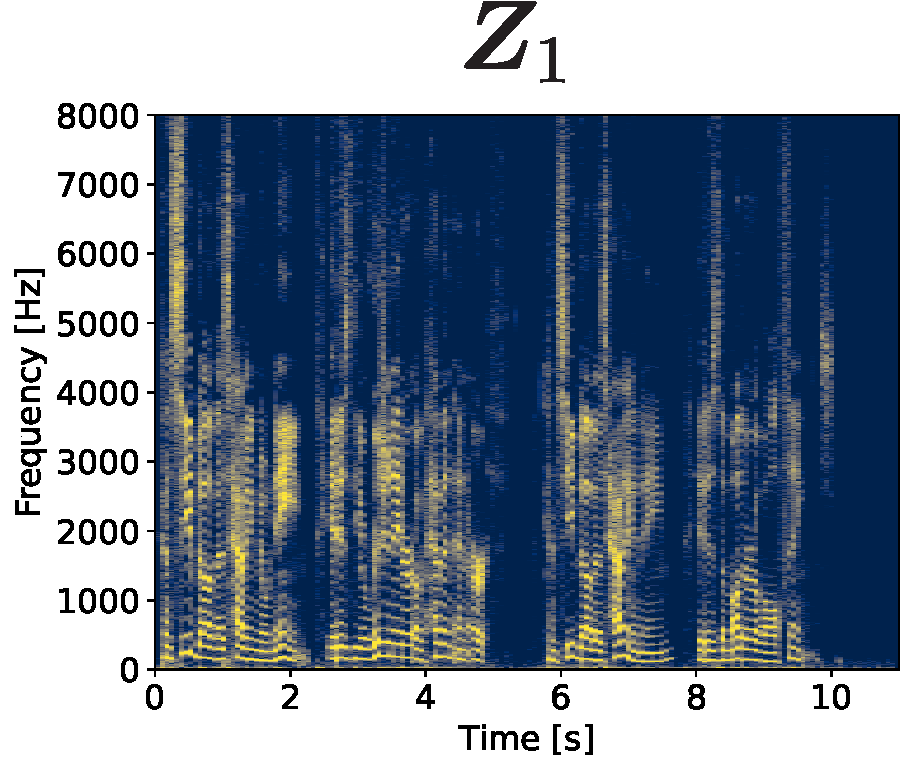
\includegraphics[keepaspectratio, scale=0.38]{figures/female_audio_spec_init.pdf}
    \subcaption{}
  \end{minipage}
  \begin{minipage}[b]{0.45\linewidth}
    \centering
    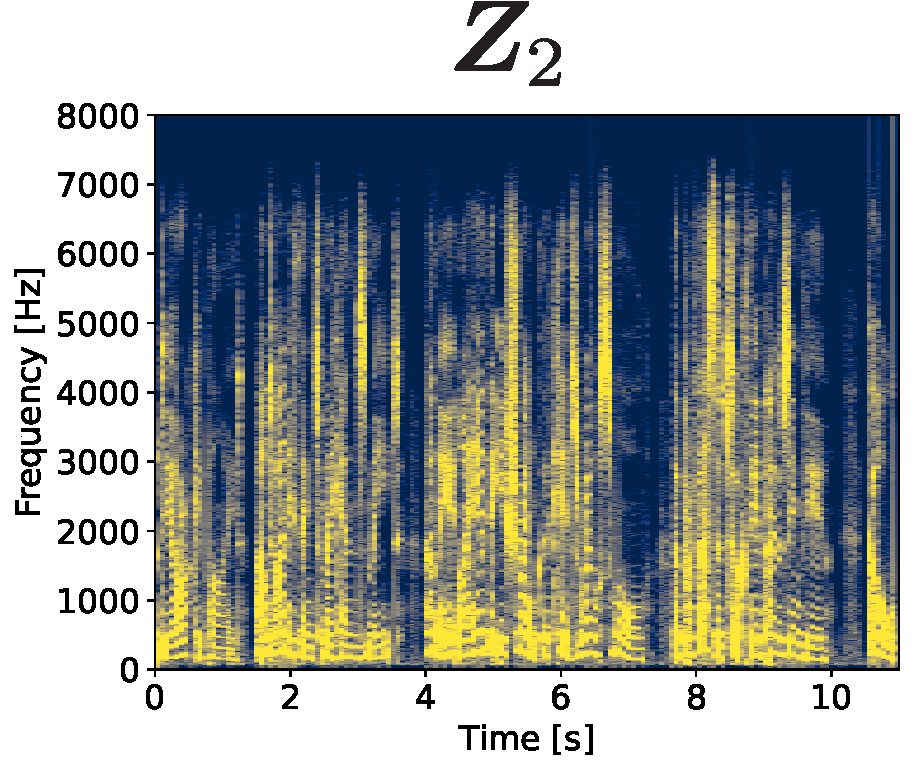
\includegraphics[keepaspectratio, scale=0.38]{figures/male_audio_spec_init.pdf}
    \subcaption{}
  \end{minipage}
  \caption{Spectrograms of speech sources: (a) female and (b) male.}
  \label{fig:audio}
\end{figure}
%%%%%%%%%%%%%%%%%%%%%%%%%%%%

%%%%%%%%%%%%%%%%%%%%%%%%%%%%
\begin{figure}[htbp]
  \begin{minipage}[b]{0.45\linewidth}
    \centering
    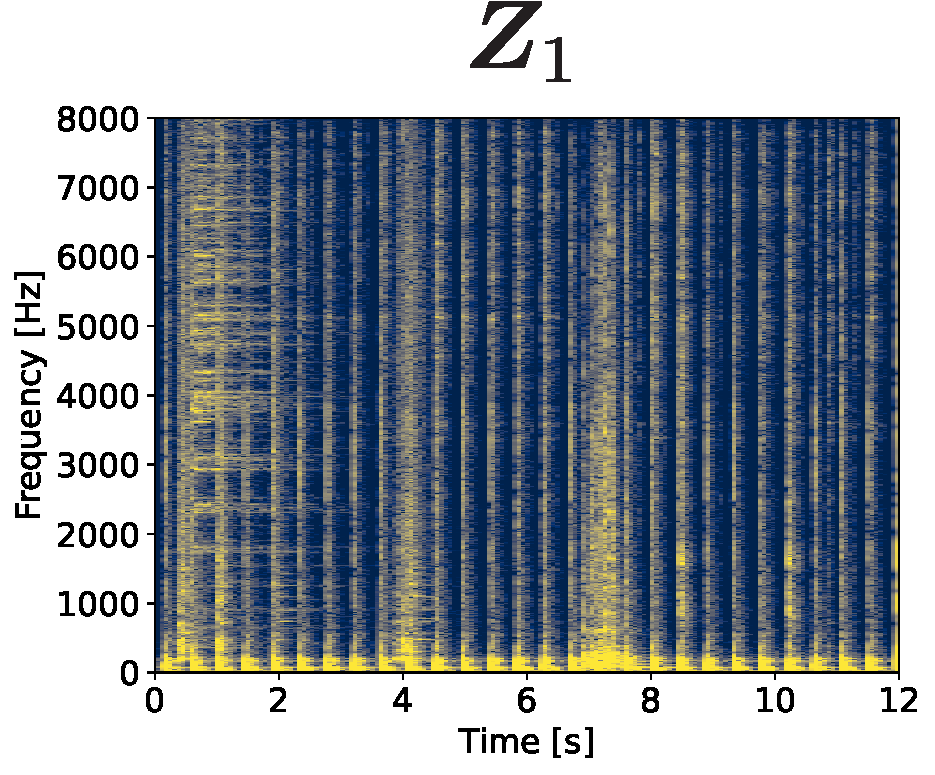
\includegraphics[keepaspectratio, scale=0.38]{figures/Drums_spec_init.pdf}
    \subcaption{}
  \end{minipage}
  \begin{minipage}[b]{0.45\linewidth}
    \centering
    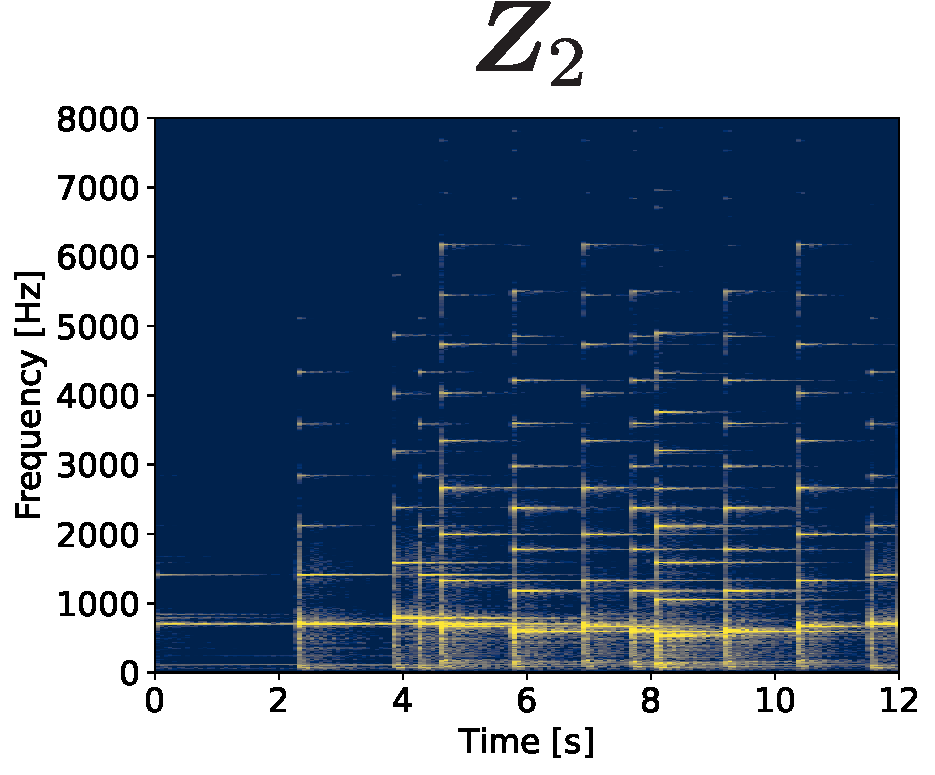
\includegraphics[keepaspectratio, scale=0.38]{figures/piano_spec_init.pdf}
    \subcaption{}
  \end{minipage}
  \caption{Spectrograms of musical instrument sources: (a) drums and (b) piano.}
  \label{fig:drum}
\end{figure}
%%%%%%%%%%%%%%%%%%%%%%%%%%%%

%----------------------------------------------

実際の音響信号を用いた実験では,パーミュテーション問題の生じていない(完全に解決された状態の)分離信号$(\bm{Z}_1, \bm{Z}_2)$として,Table~\ref{table:wav}に示す男女の音声信号及びTable~\ref{table:instrument}に示すドラムとピアノの音楽信号を用いた.
これらの信号のスペクトログラムはそれぞれFigs.~\ref{fig:audio}及び\ref{fig:drum}にそれぞれ示している.
両信号のサンプリング周波数は16~kHzであり,STFTにおける分析窓関数長(短時間信号長)を$Q=2048$点(128~ms),シフト長を$\tau=1024$点(64~ms)と設定したため,スペクトログラムのサイズは周波数ビン数が両信号ともに$I=1025$,時間フレーム数が$J=158$(音声信号)及び$J=173$(音楽信号)となった.
これらの信号を用いた実験では,IVAやILRMAで生じる可能性があるブロックパーミュテーション問題を模擬した.
具体的には,各ブロックの行数を$\gamma=16$行とし,ブロック単位でまとまって入れ替わるブロックパーミュテーション問題を模擬した推定信号$(\bm{Y}_1, \bm{Y}_2)$を生成した.
学習データ,検証データ,及びテストデータの用意やDNNの最適化の条件等については,\ref{sec:ex_condition_matrix}項と同様である.

本実験では,検証データに対する正答率に加え,SDRの改善量を用いて提案手法のパーミュテーション問題の解決性能を評価する.
SDRは,音源分離の度合と分離音の歪みの少なさの両方を加味した客観評価尺度である.
今,音源分離の目的音源信号を$\mathrm{s}(l)$,目的音以外の音源(干渉音源)信号を$\mathrm{n}(l)$とすると,これらが混合した信号$\mathrm{x}(l)$は次式となる.
\begin{align}
    \mathrm{x}(l) = \mathrm{s}(l) + \mathrm{n}(l)
\end{align}
このとき,混合信号$\mathrm{x}(l)$に音源分離を適用し得られる目的音源の推定信号$\hat{\mathrm{s}}(l)$は次式で表される.
\begin{align}
   \hat{\mathrm{s}}(l) = \mathrm{s}_{\mathrm{target}}(l) + \mathrm{e}_{\mathrm{interf}}(l) + \mathrm{e}_{\mathrm{artif}}(l)
\end{align}
ここで,$\mathrm{s}_{\mathrm{target}}(l)$,$\mathrm{e}_{\mathrm{interf}}(l)$,及び$\mathrm{e}_{\mathrm{artif}}(l)$はそれぞれ推定信号中の目的音源成分,残留した干渉音源成分,及び音源分離処理によって生じた歪み成分である.
このとき,SDRは次式のように算出できる.
\begin{align}
    \mathrm{SDR} = 10 \mathrm{log}_{10} \sum_{l=1}^L \frac{|\mathrm{s}_{\mathrm{target}}(l)|^2}{|\mathrm{e}_{\mathrm{interf}}(l) + \mathrm{e}_{\mathrm{artif}}(l)|^2}~~~\mathrm{[dB]}
\end{align}
%----------------------------------------------
\section{実験結果}
\label{sec:ex_res}
%----------------------------------------------
%----------------------------------------------
\subsection{人工データに対する実験結果}
\label{sec:ex_res_artificial}
%----------------------------------------------

Figs.~\ref{fig:01mat_1block}--\ref{fig:stripe_1block}にそれぞれ,Figs.~\ref{fig:01mat_spec}--\ref{fig:stripe_spec}の人工データ行列に対して1行毎にランダムに入れ替える場合($\gamma=1$)の実験結果を示している.
この結果では,学習時の学習データ及び検証データに対する正答率(各図における(a))と検証データの入力及び予測結果(各図における(b))をそれぞれ示している.
この結果を見ると,Figs.~\ref{fig:01mat_spec}及び\ref{fig:25stripe_spec}に示すような単純な構造を持つ行列に対しては,Figs.~\ref{fig:01mat_1block} (a)及び\ref{fig:25mat_1block} (a)に示すようにいずれも検証データに対する正答率が100\%に近い値となっている.
予測結果であるFigs.~\ref{fig:01mat_1block} (b)及び\ref{fig:25mat_1block} (b)の推定分離信号$(\hat{\bm{Z}}_1, \hat{\bm{Z}}_2)$は少しの間違いを含んでいるものの,高精度で正しい並び替えができていることが分かる.
しかしながら,Fig.~\ref{fig:stripe_spec}に示す1列毎に0と1の値が入れ替わる行列に対しては,Fig.~\ref{fig:stripe_1block} (a)に示すように検証データに対する正答率が54\%程度となった.
予測結果であるFig.~\ref{fig:stripe_1block} (b)の推定分離信号$(\hat{\bm{Z}}_1, \hat{\bm{Z}}_2)$を見ても正しい並び替えができていないことが分かる.

次に,Figs.~\ref{fig:01mat_2block}--\ref{fig:stripe_2block}にそれぞれFigs.~\ref{fig:01mat_spec}--\ref{fig:stripe_spec}の人工データ行列に対して2行毎にランダムに入れ替える場合($\gamma=2$)の実験結果を示している.
Figs.~\ref{fig:01mat_1block}--\ref{fig:stripe_1block}と同様に,学習時の学習データ及び検証データに対する正答率(各図における(a))と検証データの入力及び予測結果(各図における(b))をそれぞれ示している.
これらの結果では,どの実験結果においても検証データに対する正答率が90\%を超えており,推定分離信号$(\hat{\bm{Z}}_1, \hat{\bm{Z}}_2)$も高精度で正しい並び替えが達成できていることが確認できる.
さらにブロックパーミュテーション問題におけるブロックサイズを大きくした$\gamma=4$及び$\gamma=8$の結果についても付録\ref{chap:artificial}に掲載している.
いずれも検証データに対して高い正答率を達成している.
これらの結果から分かることとして,提案手法の深層パーミュテーション解決法はブロックサイズが$\gamma=2$以上のブロックパーミュテーション問題であれば,複雑な構造を持つ音源信号に対しても高精度に解決することができる可能性が高い.
一方で,周波数ビン毎に推定信号の順序がランダムに入れ替える一般的なパーミュテーション問題について解決は精度の低下が見られるため,FDICAの推定信号に対してそのまま提案手法を適用することは効果的ではない可能性がある.

%%%%%%%%%%%%%%%%%%%%%%%%%%%%
\begin{figure*}[!t]
    \centering
    \subfloat[Accuracy for training and validation data.]{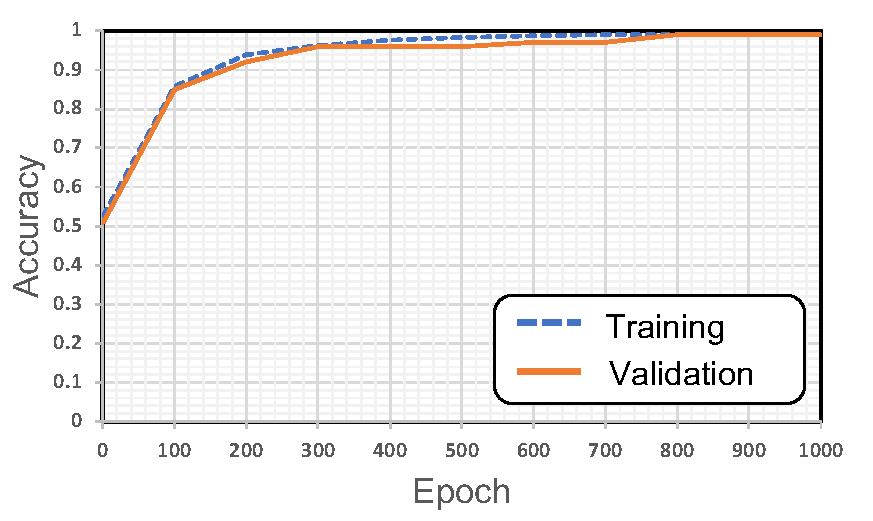
\includegraphics[clip, width=4.5in]{figures/graph/01mat_1block.pdf}
    \vspace{-15pt}
    \label{fig:acc_01mat_1block}}
    \\
    \subfloat[Input matrices with permutation problem (upper) and permutation-aligned matrices using predicted results (bottom).]{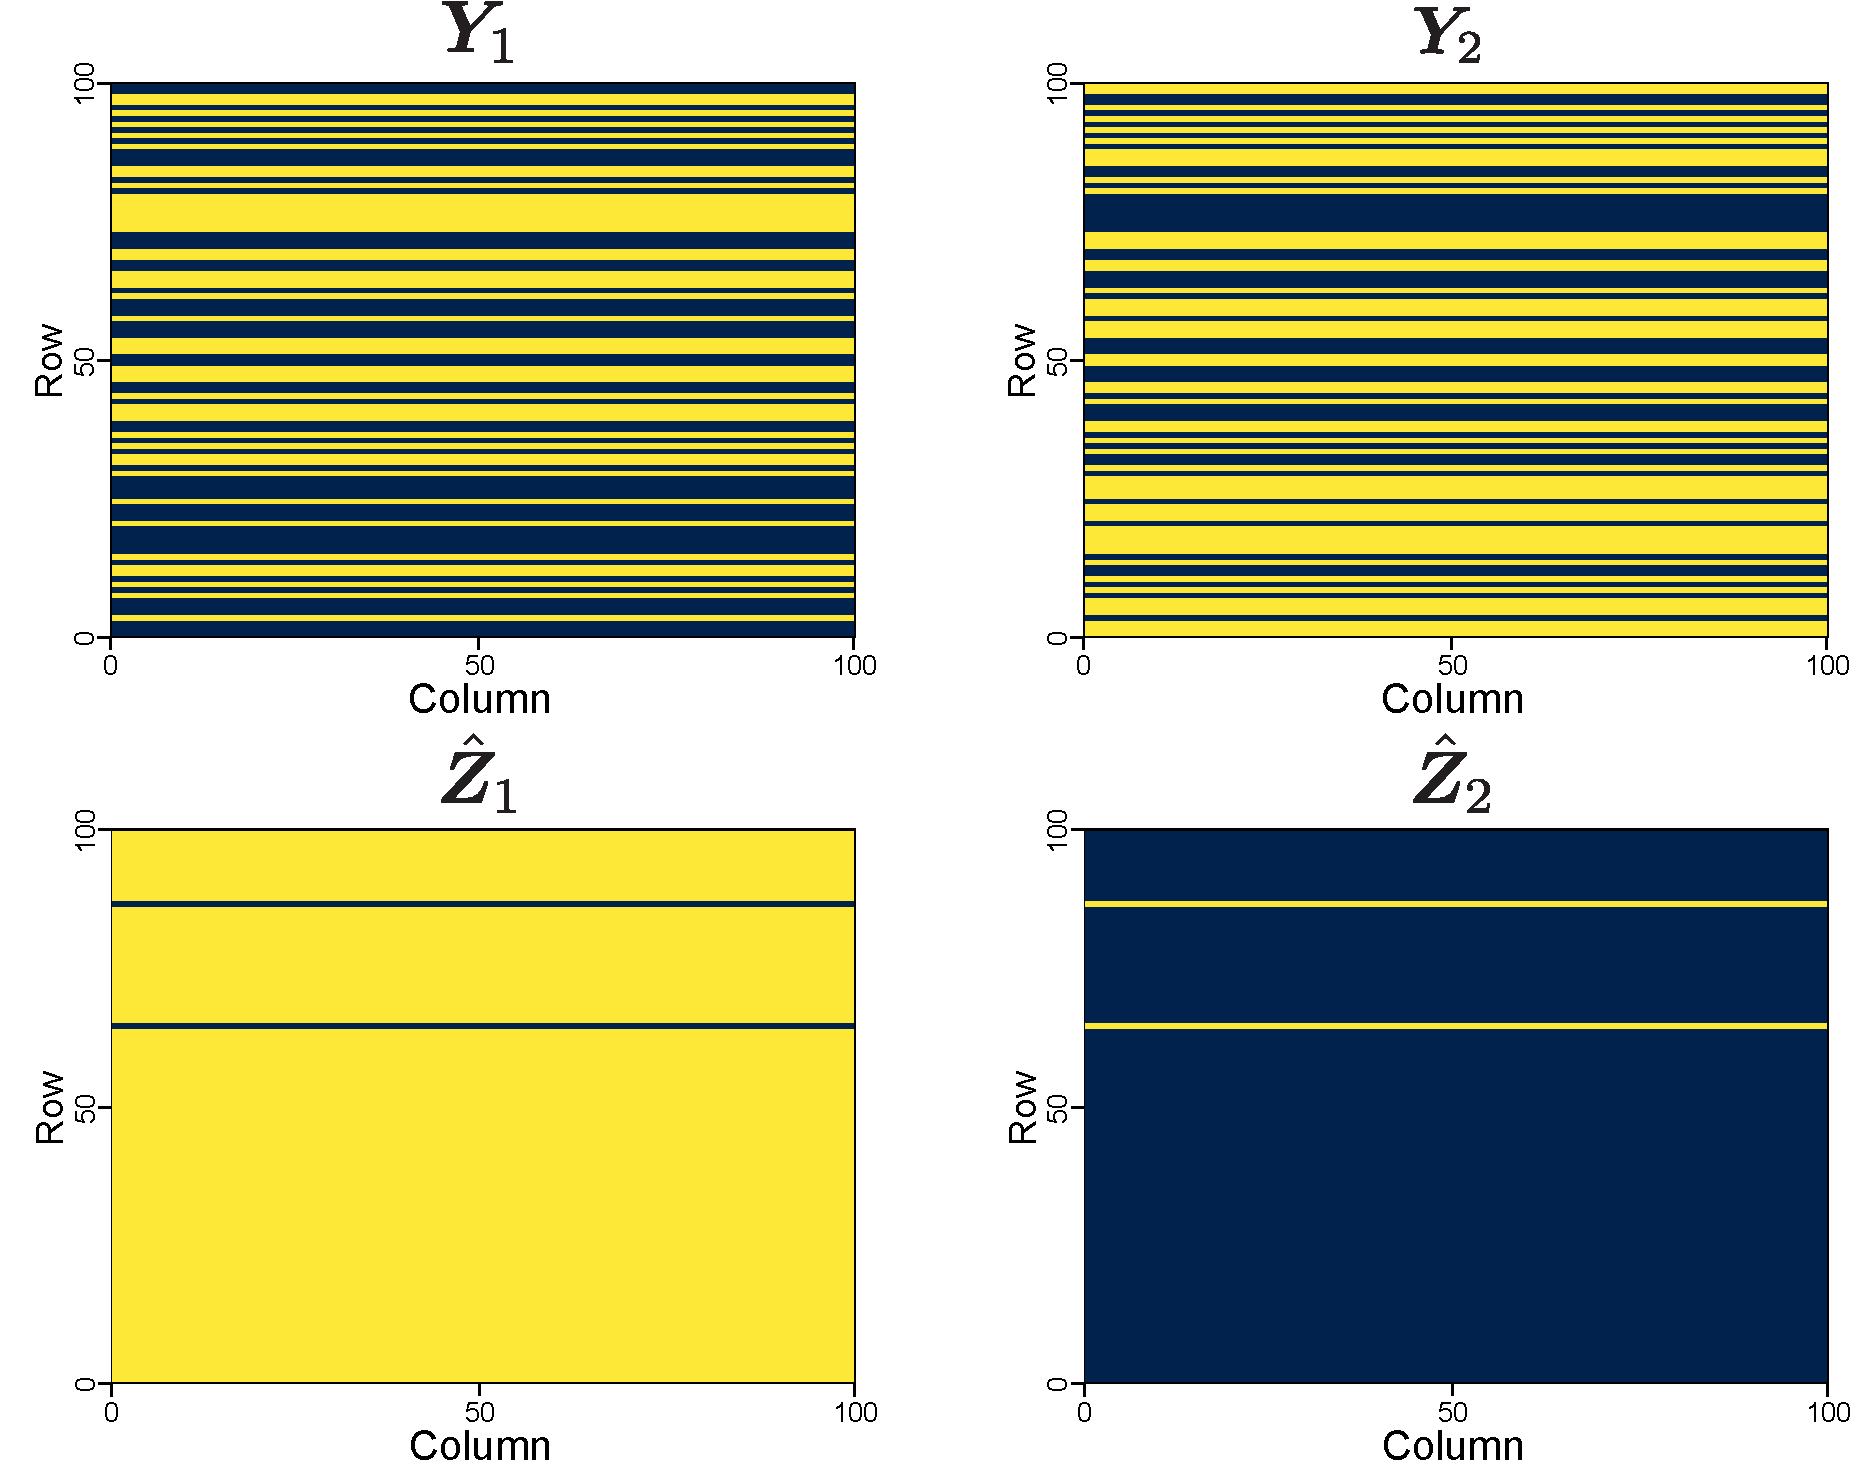
\includegraphics[clip, width=5.0in]{figures/01mat_1block.pdf}
    \label{fig:spec_01mat_1block}}  
    \caption{Experimental results with $\gamma=1$ using artificial source matrices of Fig.~\ref{fig:01mat_spec}.}
    \label{fig:01mat_1block}
\end{figure*}
%%%%%%%%%%%%%%%%%%%%%%%%%%%%

%%%%%%%%%%%%%%%%%%%%%%%%%%%%
\begin{figure*}[!t]
    \centering
    \subfloat[Accuracy for training and validation data.]{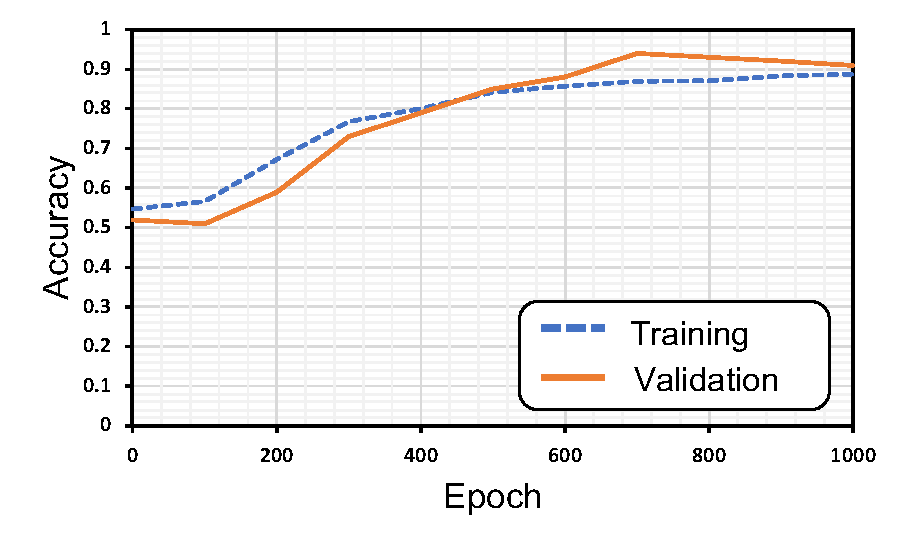
\includegraphics[clip, width=4.5in]{figures/graph/graph_25stripe_1block.pdf}
    \vspace{-15pt}
    \label{fig:acc_25mat_1block}}
    \\
    \subfloat[Input matrices with permutation problem (upper) and permutation-aligned matrices using predicted results (bottom).]{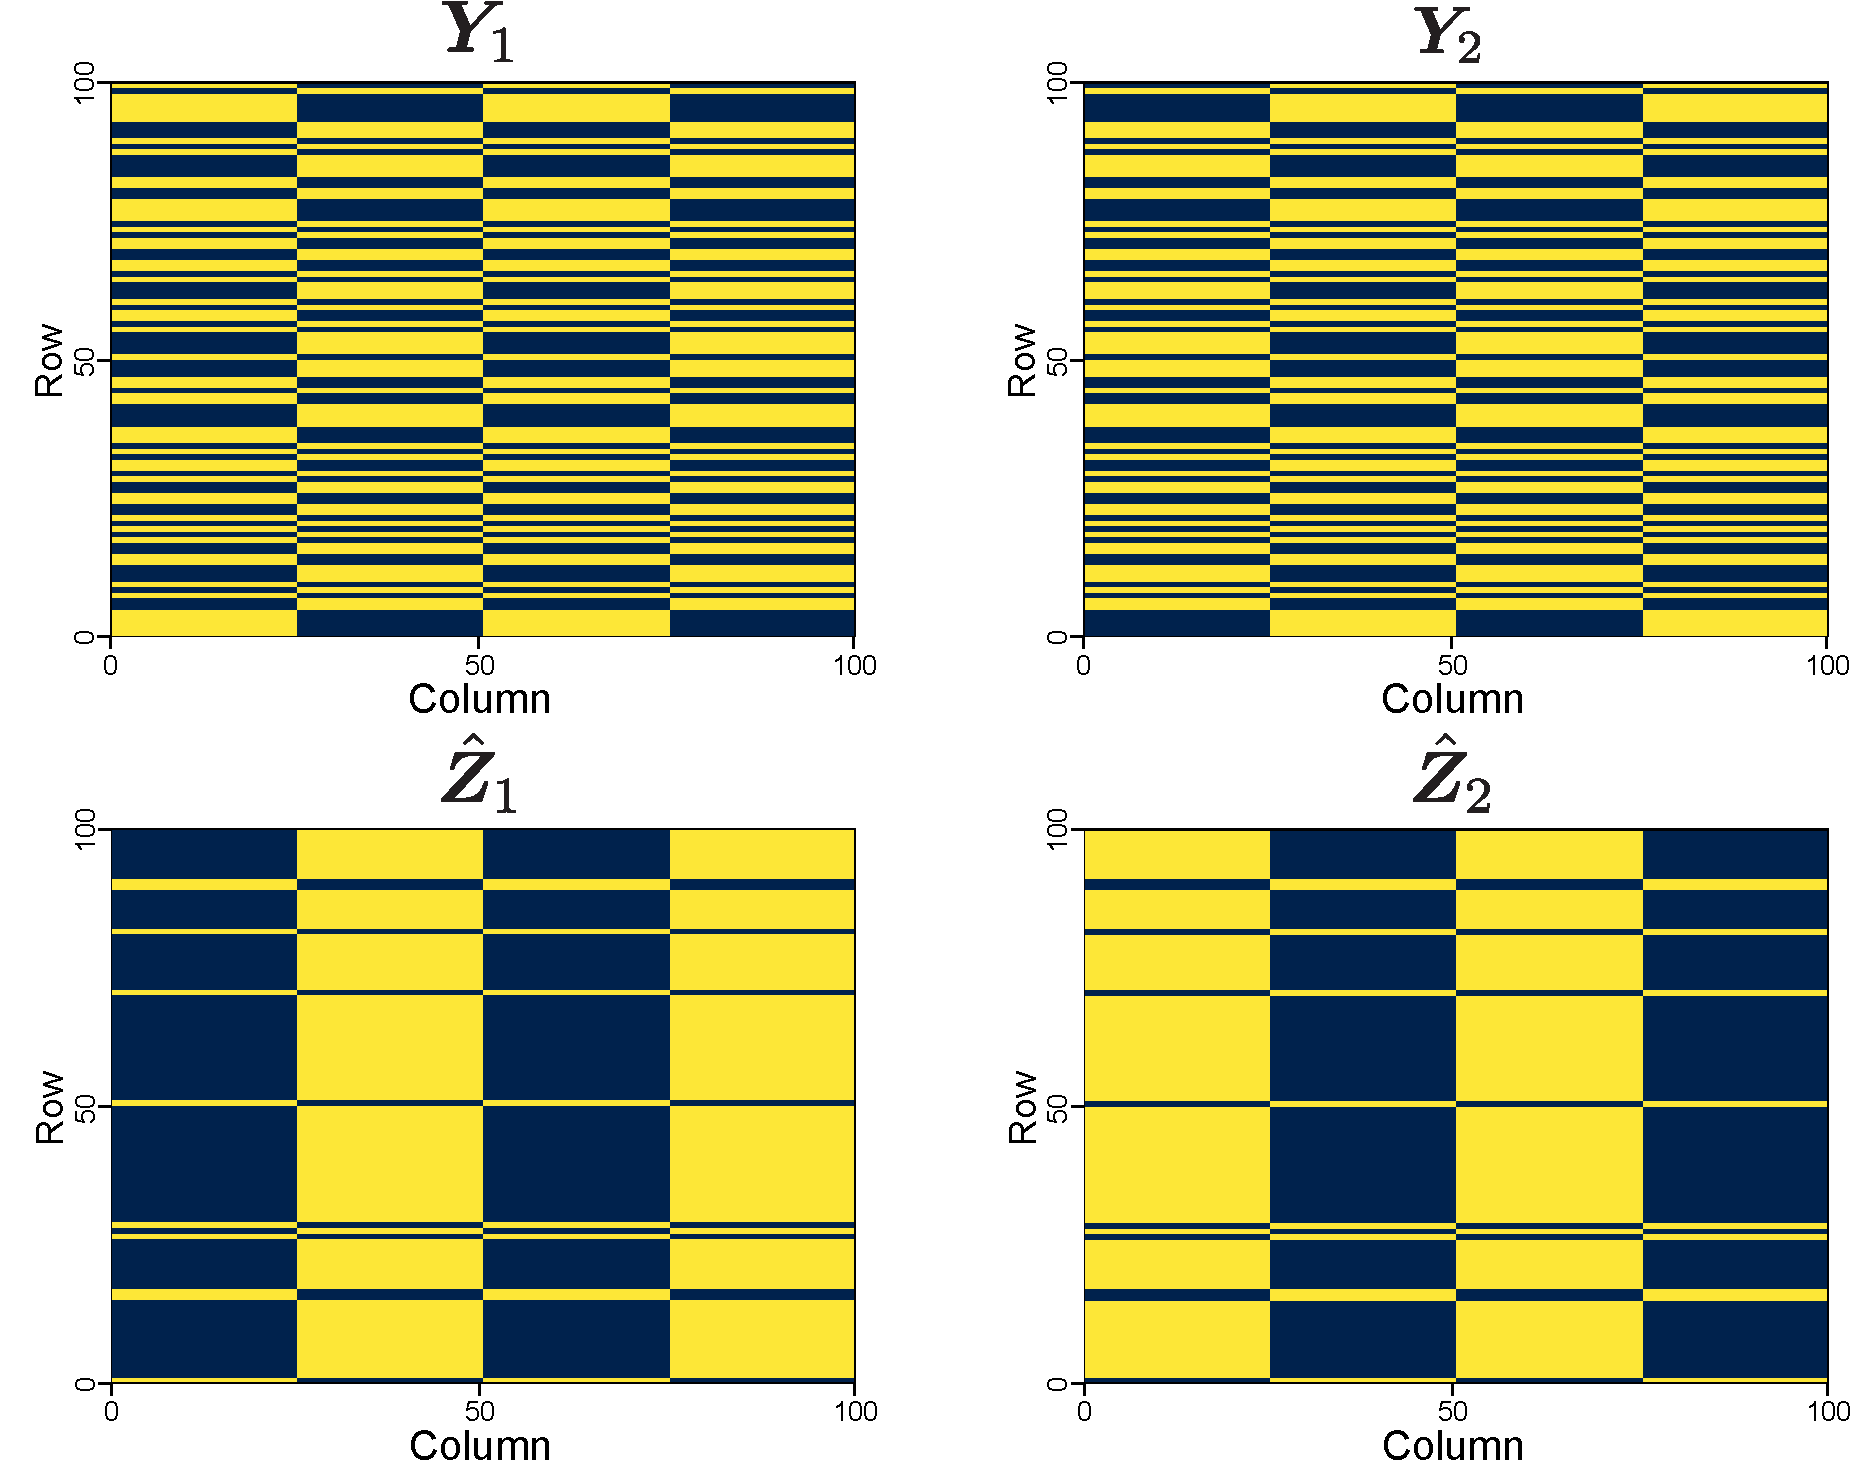
\includegraphics[clip, width=5.0in]{figures/25stripe_1block.pdf}
    \label{fig:spec_25mat_1block}}  
    \caption{Experimental results with $\gamma=1$ using artificial source matrices of Fig.~\ref{fig:25stripe_spec}.}
    \label{fig:25mat_1block}
\end{figure*}
%%%%%%%%%%%%%%%%%%%%%%%%%%%%

%%%%%%%%%%%%%%%%%%%%%%%%%%%%
\begin{figure*}[!t]
    \centering
    \subfloat[Accuracy for training and validation data.]{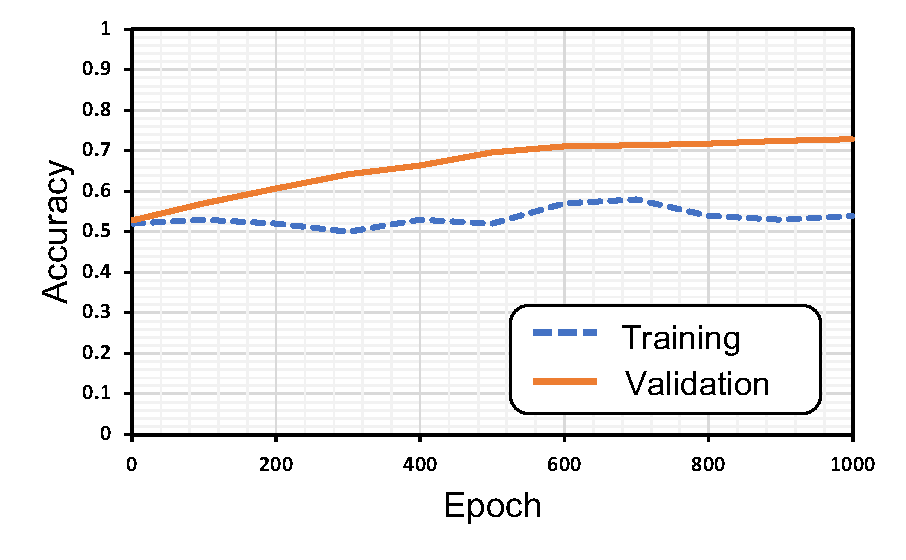
\includegraphics[clip, width=4.5in]{figures/graph/graph_stripe_1block.pdf}
    \vspace{-15pt}
    \label{fig:acc_stripe_1block}}
    \\
    \subfloat[Input matrices with permutation problem (upper) and permutation-aligned matrices using predicted results (bottom).]{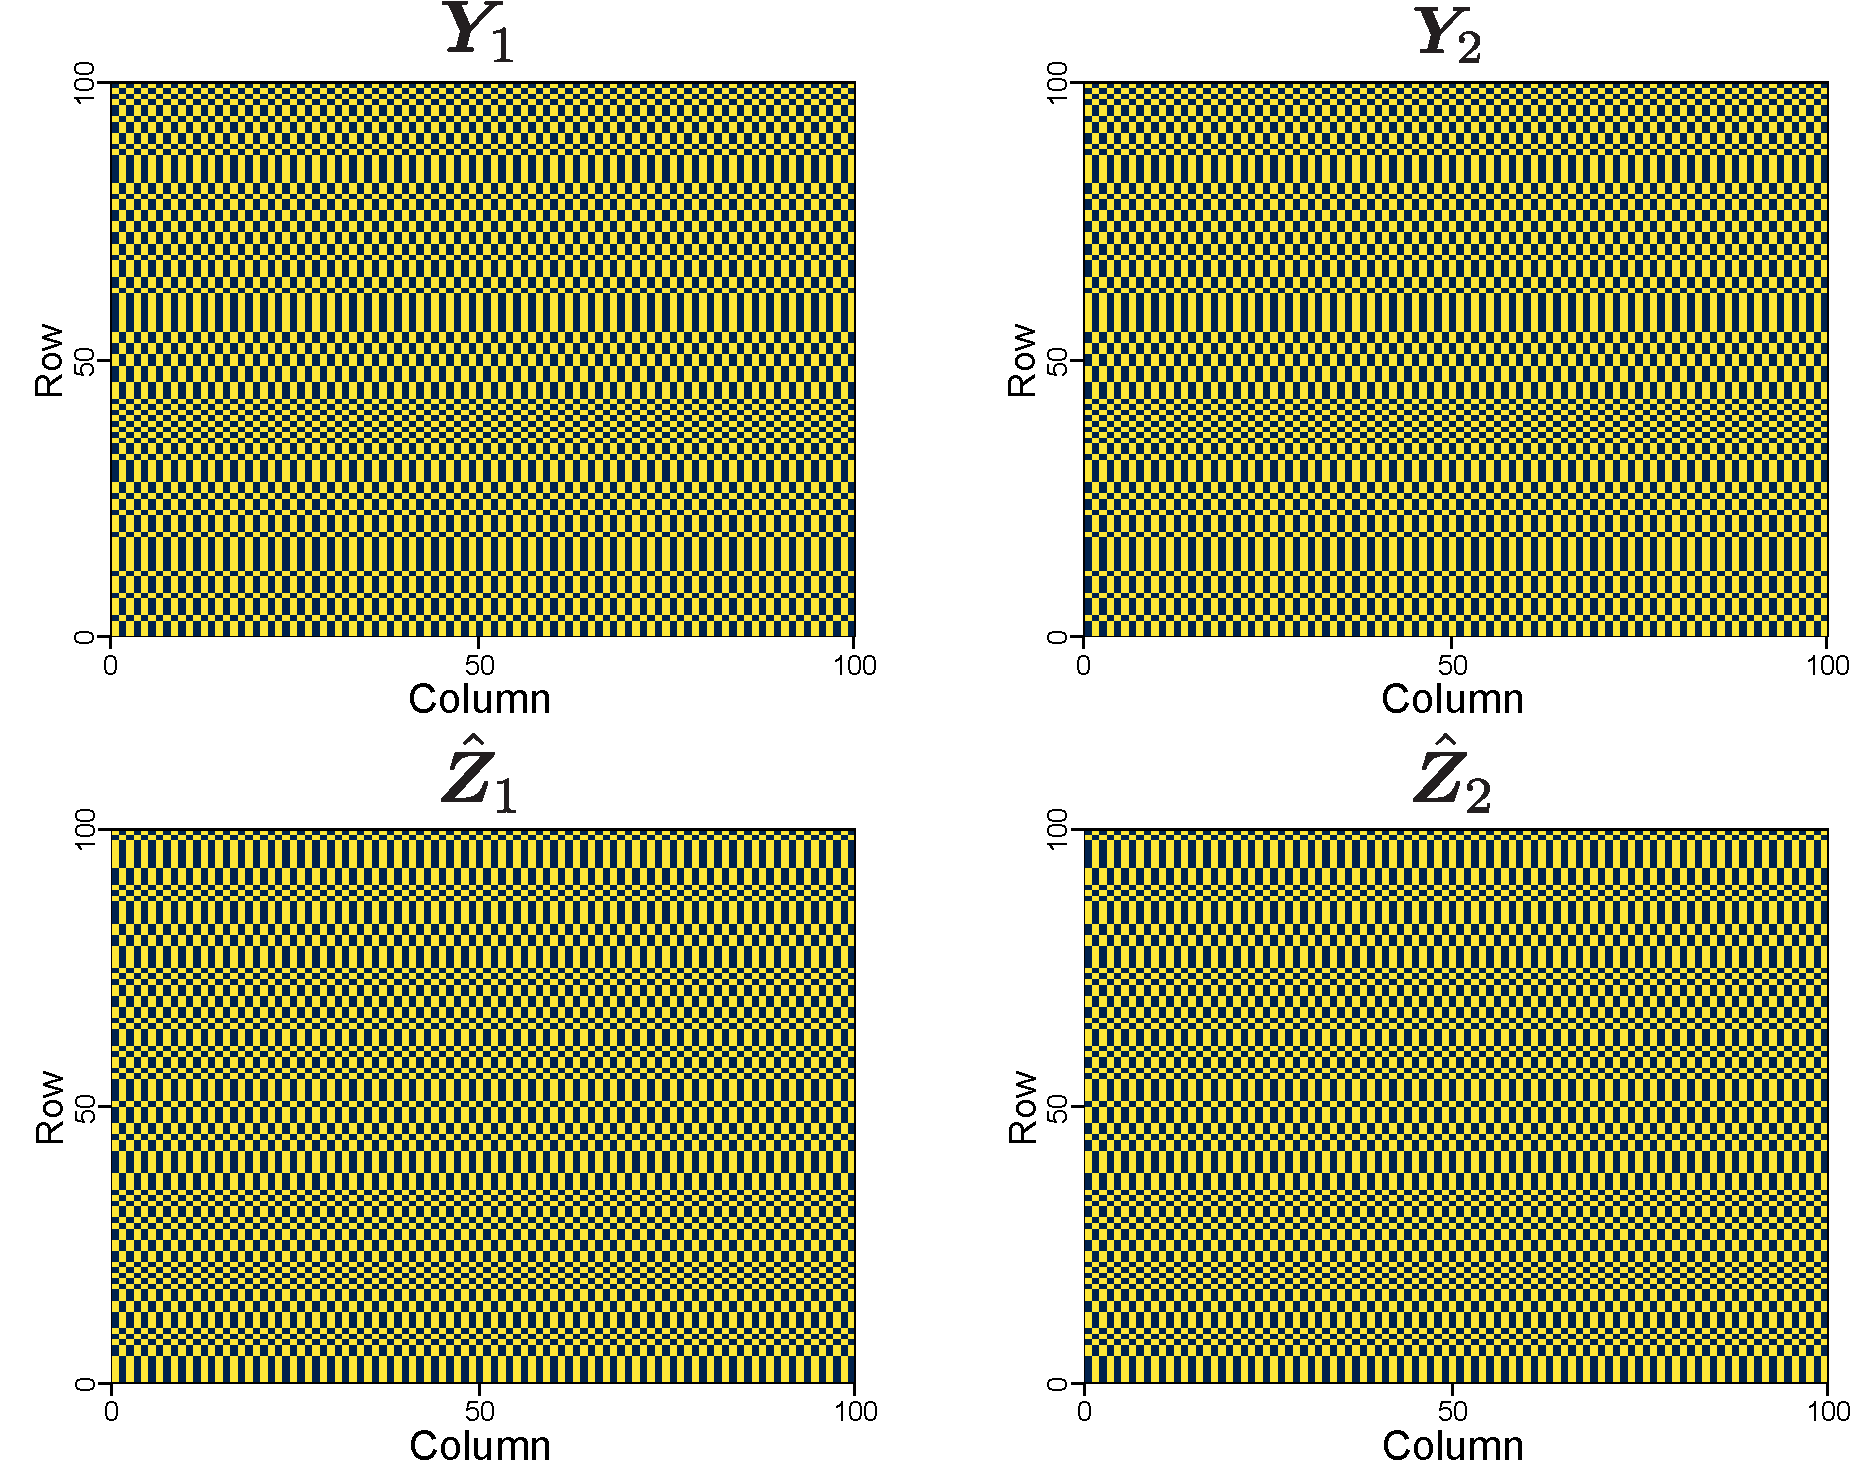
\includegraphics[clip, width=5.0in]{figures/stripe_1block.pdf}
    \label{fig:spec_stripe_1block}}  
    \caption{Experimental results with $\gamma=1$ using artificial source matrices of Fig.~\ref{fig:stripe_spec}.}
    \label{fig:stripe_1block}
\end{figure*}
%%%%%%%%%%%%%%%%%%%%%%%%%%%%

%%%%%%%%%%%%%%%%%%%%%%%%%%%%
\begin{figure*}[!t]
  \centering
  \subfloat[Accuracy for training and validation data.]{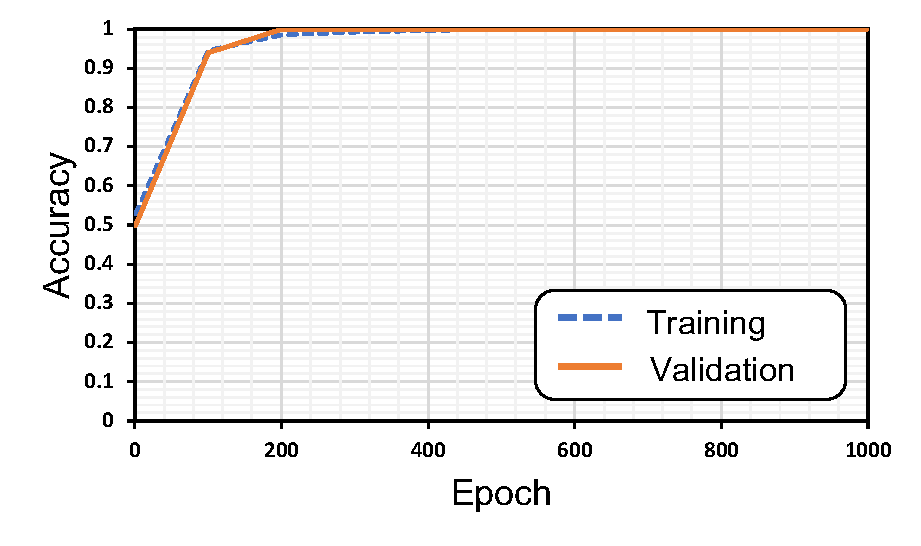
\includegraphics[clip, width=4.5in]{figures/graph/01mat_2block.pdf}
  \vspace{-15pt}
  \label{fig:acc_01mat_2block}}
  \\
  \subfloat[Input matrices with permutation problem (upper) and permutation-aligned matrices using predicted results (bottom).]{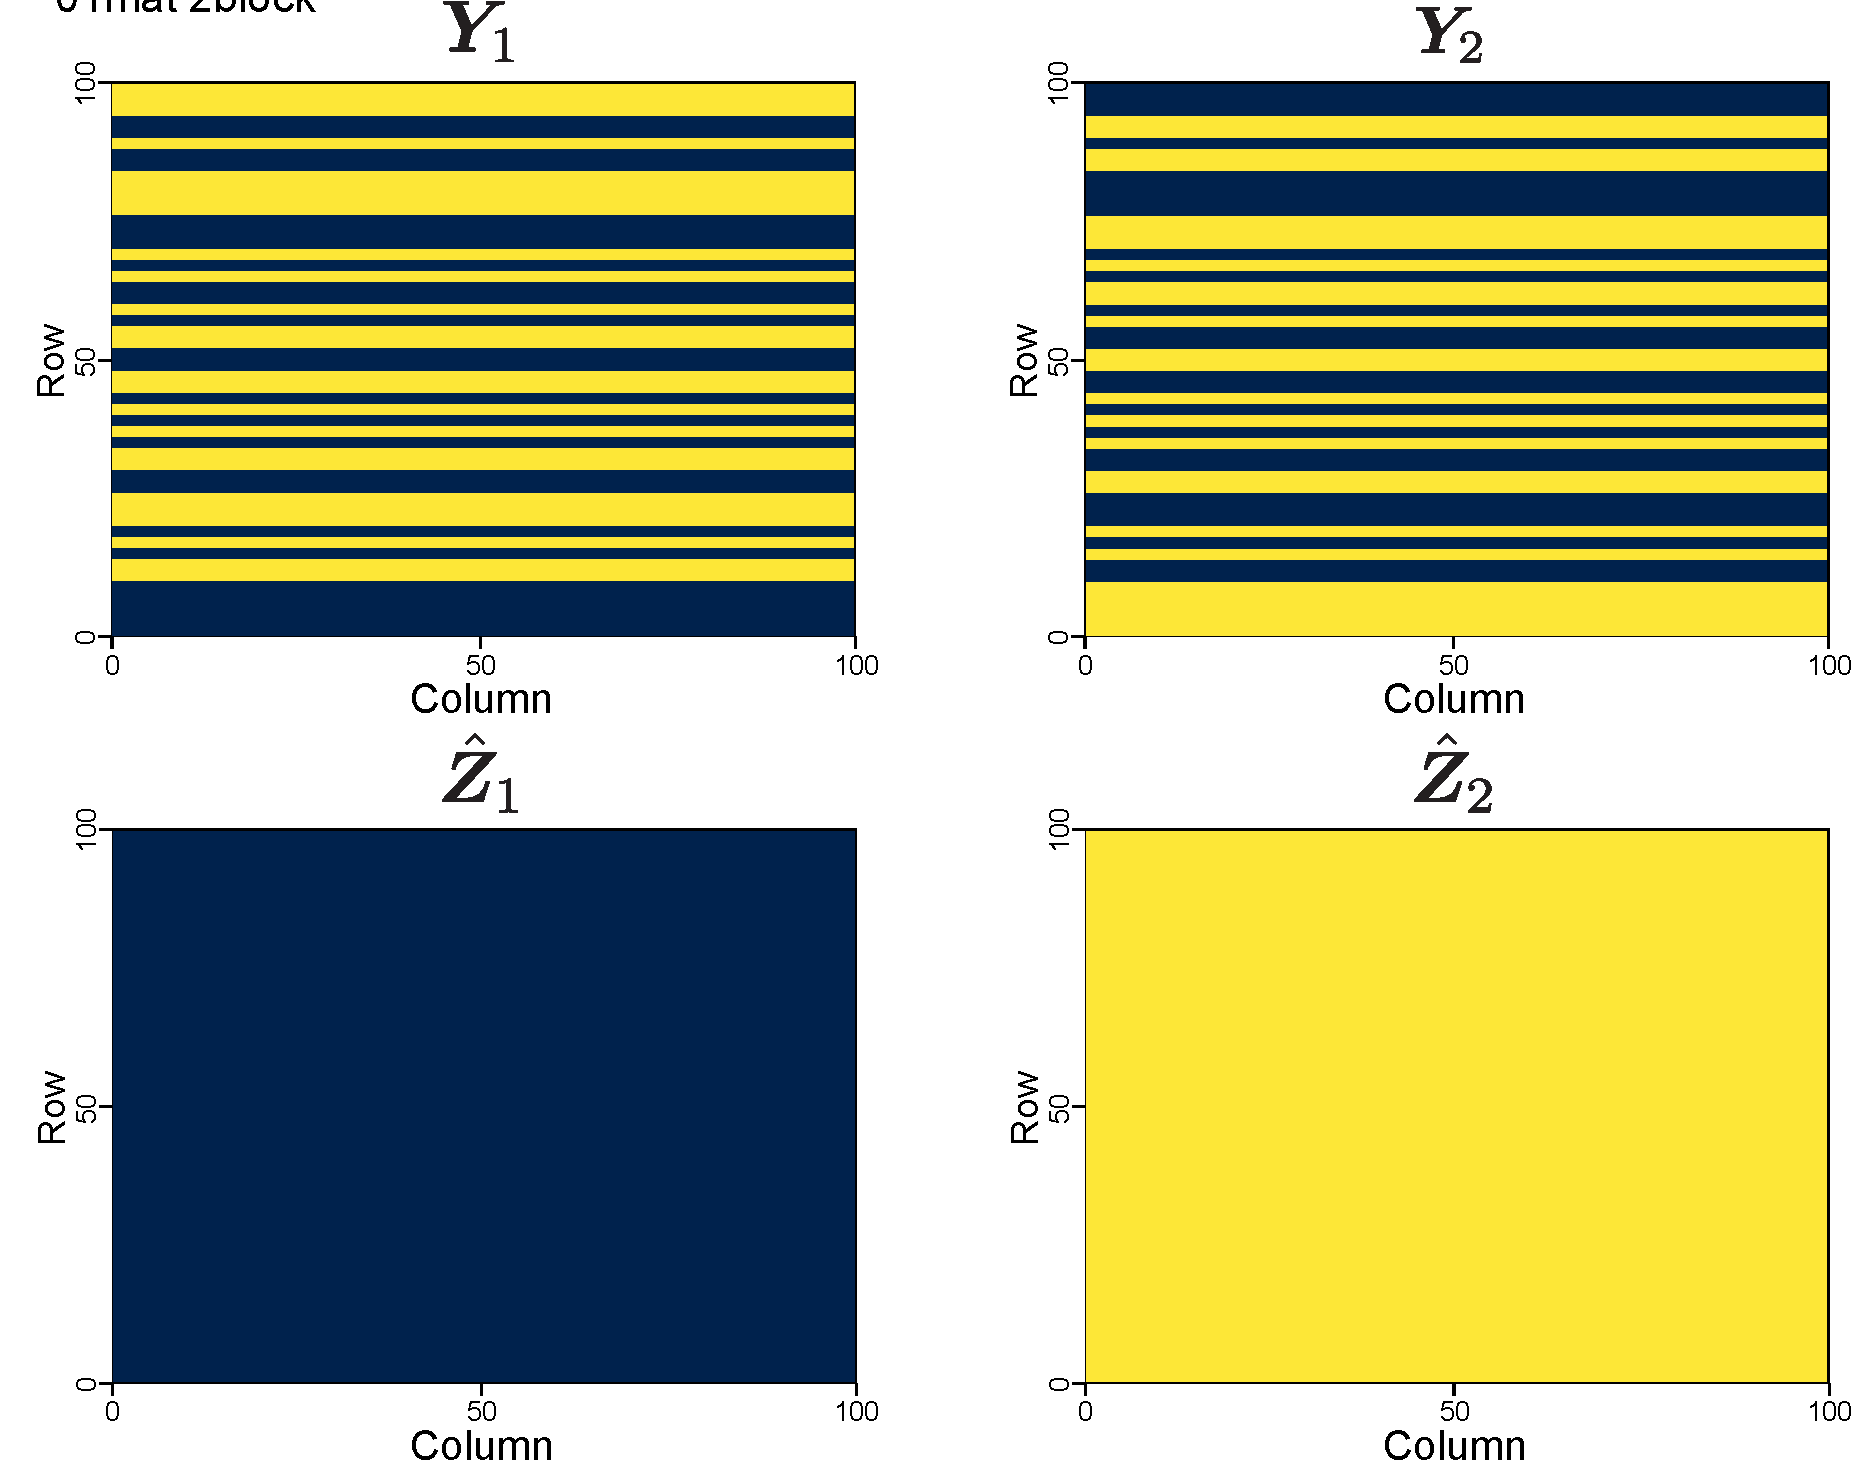
\includegraphics[clip, width=5.0in]{figures/01mat_2block.pdf}
  \label{fig:spec_01mat_2block}}
  \caption{Experimental results with $\gamma=2$ using artificial source matrices of Fig.~\ref{fig:01mat_spec}.}
  \label{fig:01mat_2block}
\end{figure*}
%%%%%%%%%%%%%%%%%%%%%%%%%%%%

%%%%%%%%%%%%%%%%%%%%%%%%%%%%
\begin{figure*}[!t]
  \centering
  \subfloat[Accuracy for training and validation data.]{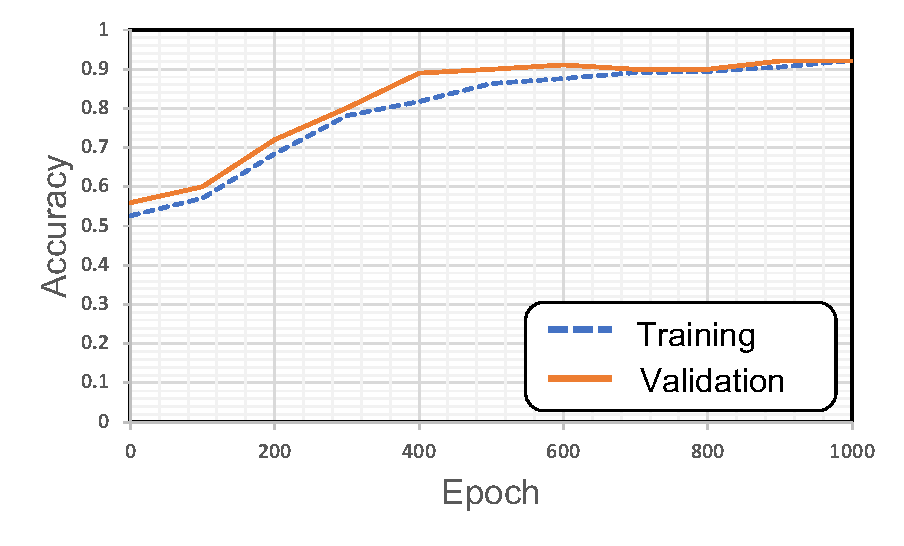
\includegraphics[clip, width=4.5in]{figures/graph/25stripe_2block.pdf}
  \vspace{-15pt}
  \label{fig:acc_25stripe_2block}}
  \\
  \subfloat[Input matrices with permutation problem (upper) and permutation-aligned matrices using predicted results (bottom).]{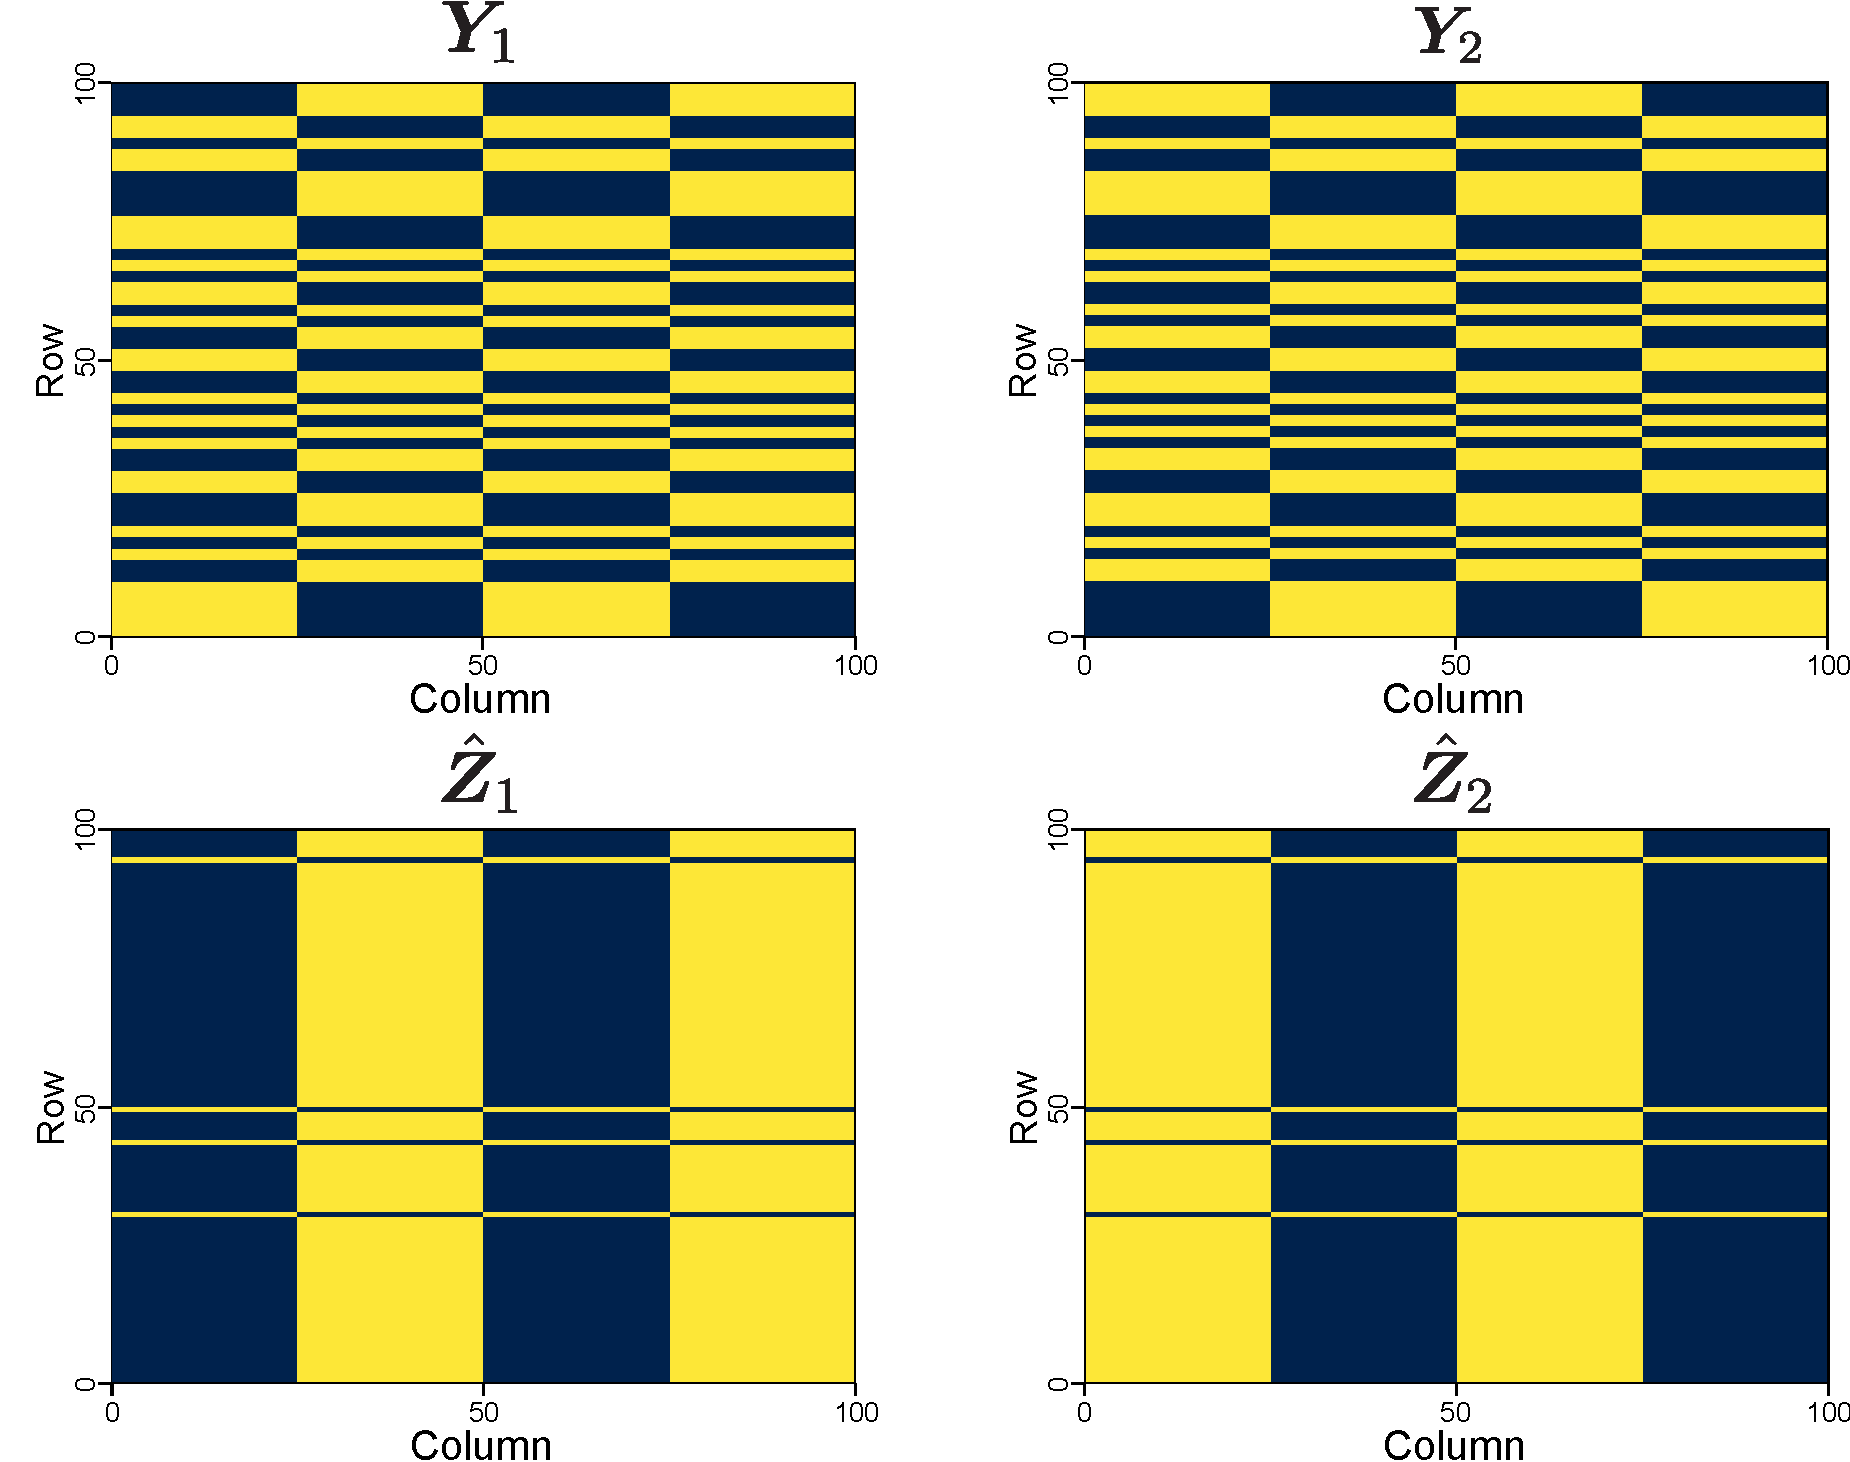
\includegraphics[clip, width=5.0in]{figures/25stripe_2block.pdf}
  \label{fig:spec_25stripe_2block}}
  \caption{Experimental results with $\gamma=2$ using artificial source matrices of Fig.~\ref{fig:25stripe_spec}.}
  \label{fig:25stripe_2block}
\end{figure*}
%%%%%%%%%%%%%%%%%%%%%%%%%%%%

%%%%%%%%%%%%%%%%%%%%%%%%%%%%
\begin{figure*}[!t]
  \centering
  \subfloat[Accuracy for training and validation data.]{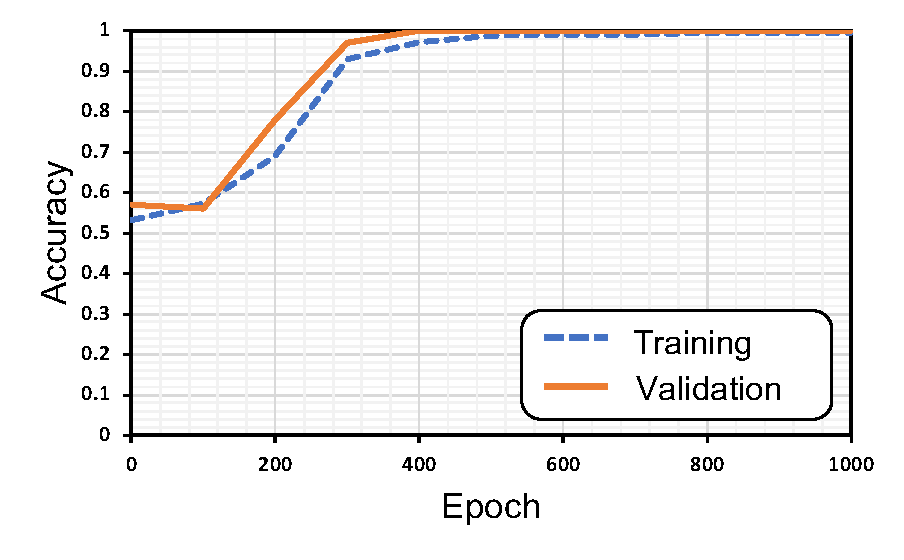
\includegraphics[clip, width=4.5in]{figures/graph/stripe_2block.pdf}
  \vspace{-15pt}
  \label{fig:acc_stripe_2block}}
  \\
  \subfloat[Input matrices with permutation problem (upper) and permutation-aligned matrices using predicted results (bottom).]{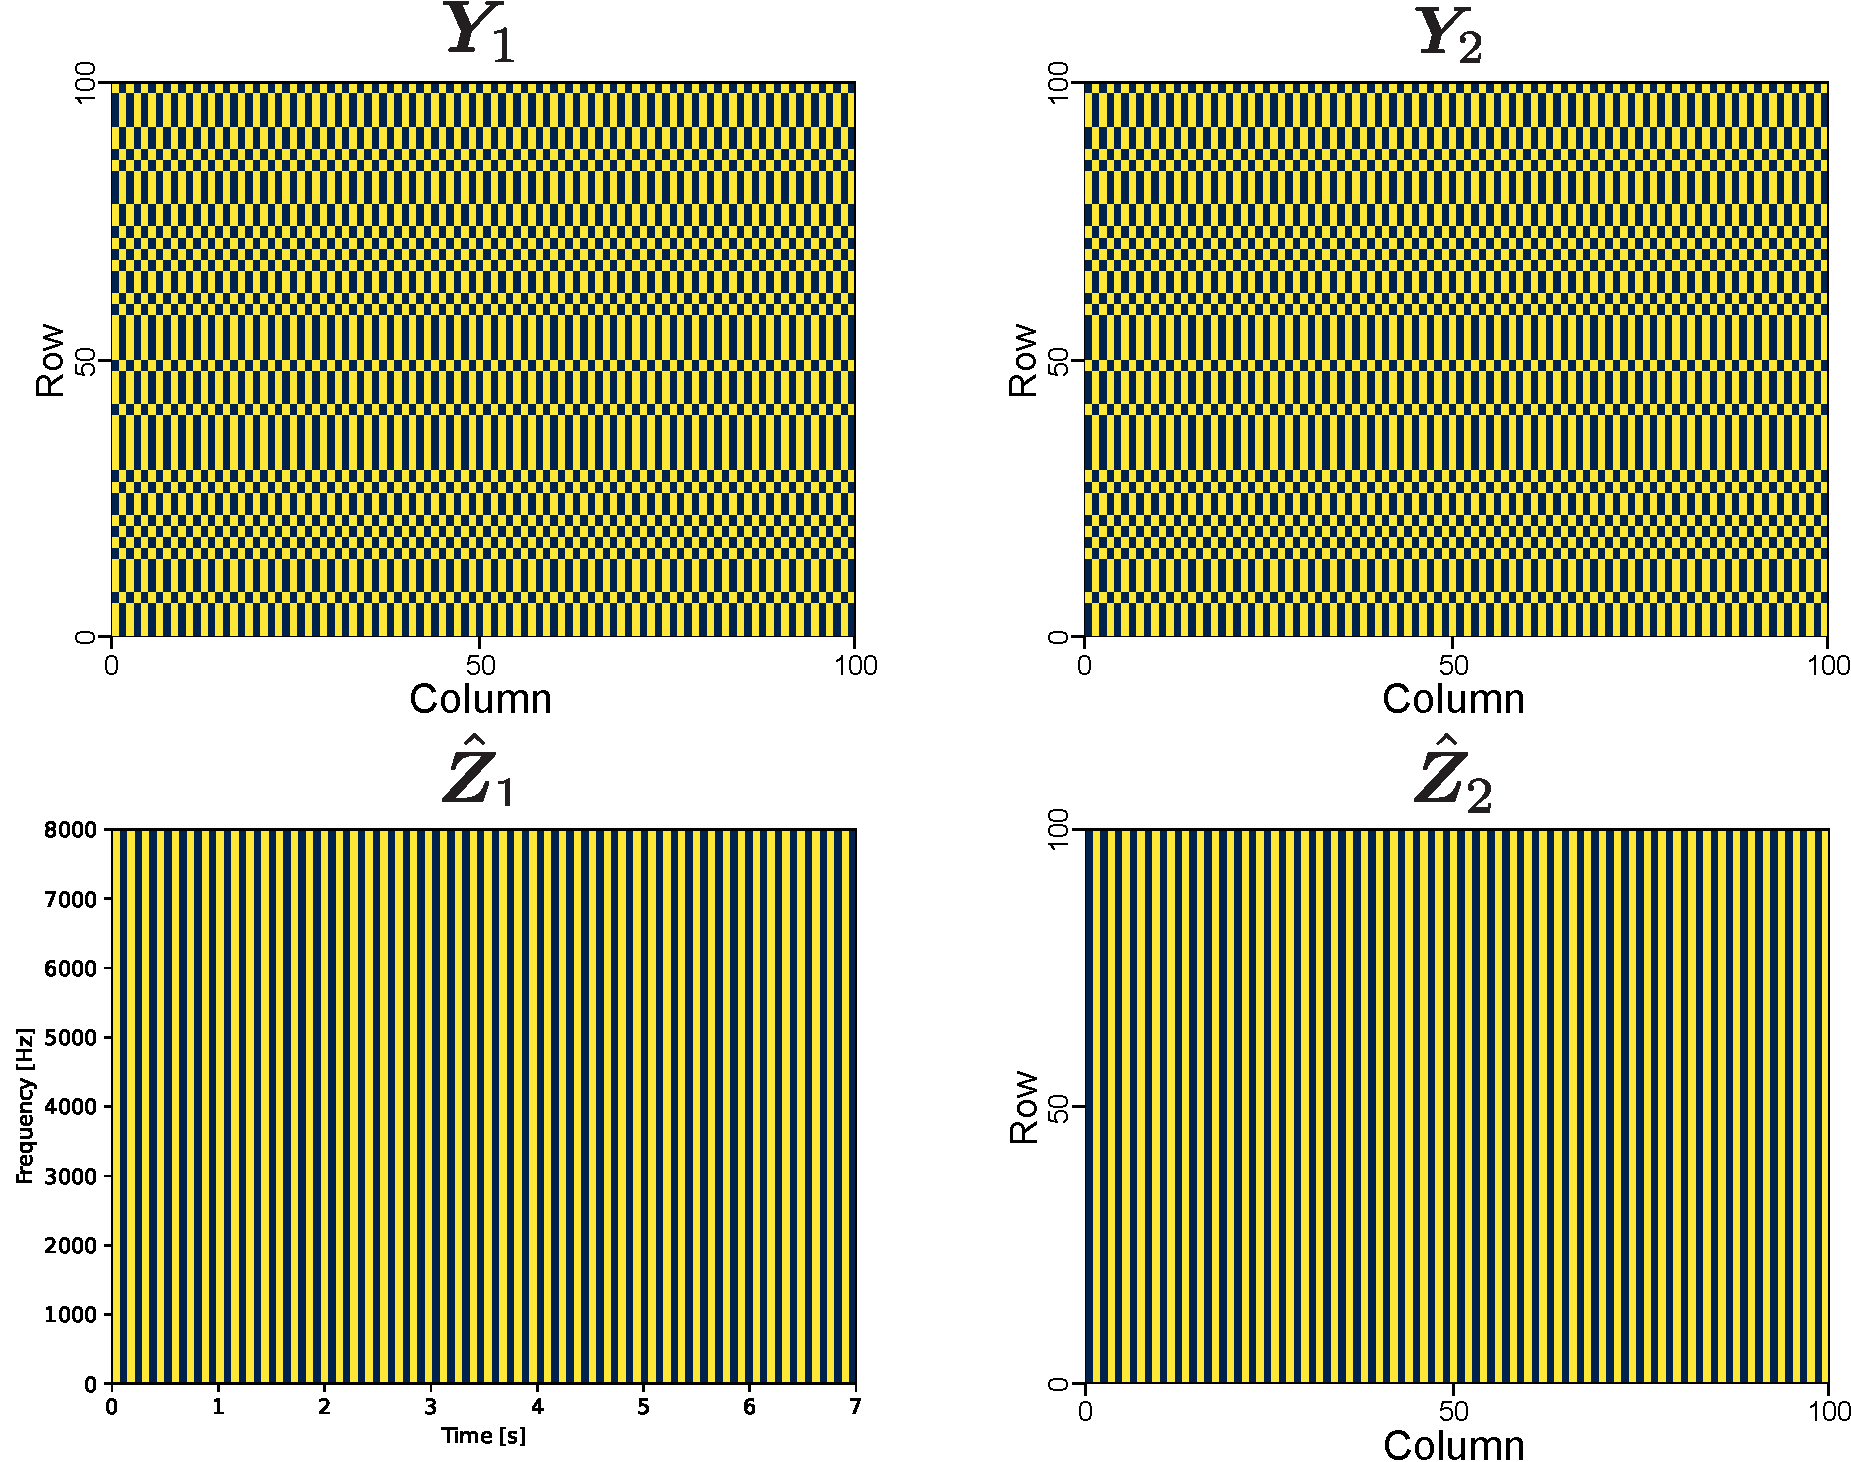
\includegraphics[clip, width=5.0in]{figures/stripe_2block.pdf}
  \label{fig:spec_stripe_2block}}
  \caption{Experimental results with $\gamma=2$ using artificial source matrices of Fig.~\ref{fig:stripe_spec}.}
  \label{fig:stripe_2block}
\end{figure*}
%%%%%%%%%%%%%%%%%%%%%%%%%%%%


\clearpage
%----------------------------------------------
\subsection{音声及び音楽信号に対する実験結果}
\label{sec:ex_res_artificial}
%----------------------------------------------

%%%%%%%%%%%%%%%%%%%%%%%%%%%%
\begin{figure*}[!t]
  \centering
  \subfloat[Accuracy for training and validation data.]{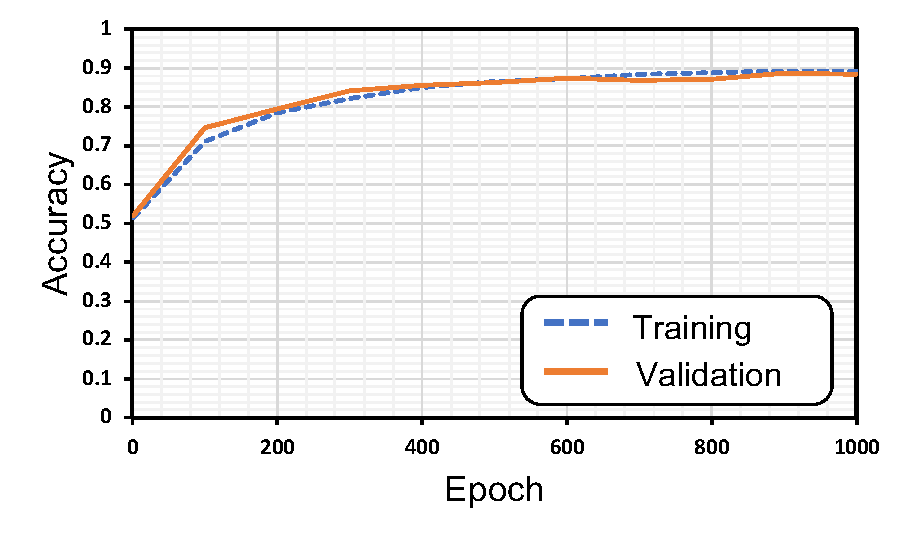
\includegraphics[clip, width=4.5in]{figures/graph/audio_16block.pdf}
  \vspace{-15pt}
  \label{fig:acc_audio_16block}}
  \\
  \subfloat[Input spectrograms with permutation problem (upper) and permutation-aligned spectrograms using predicted results (bottom).]{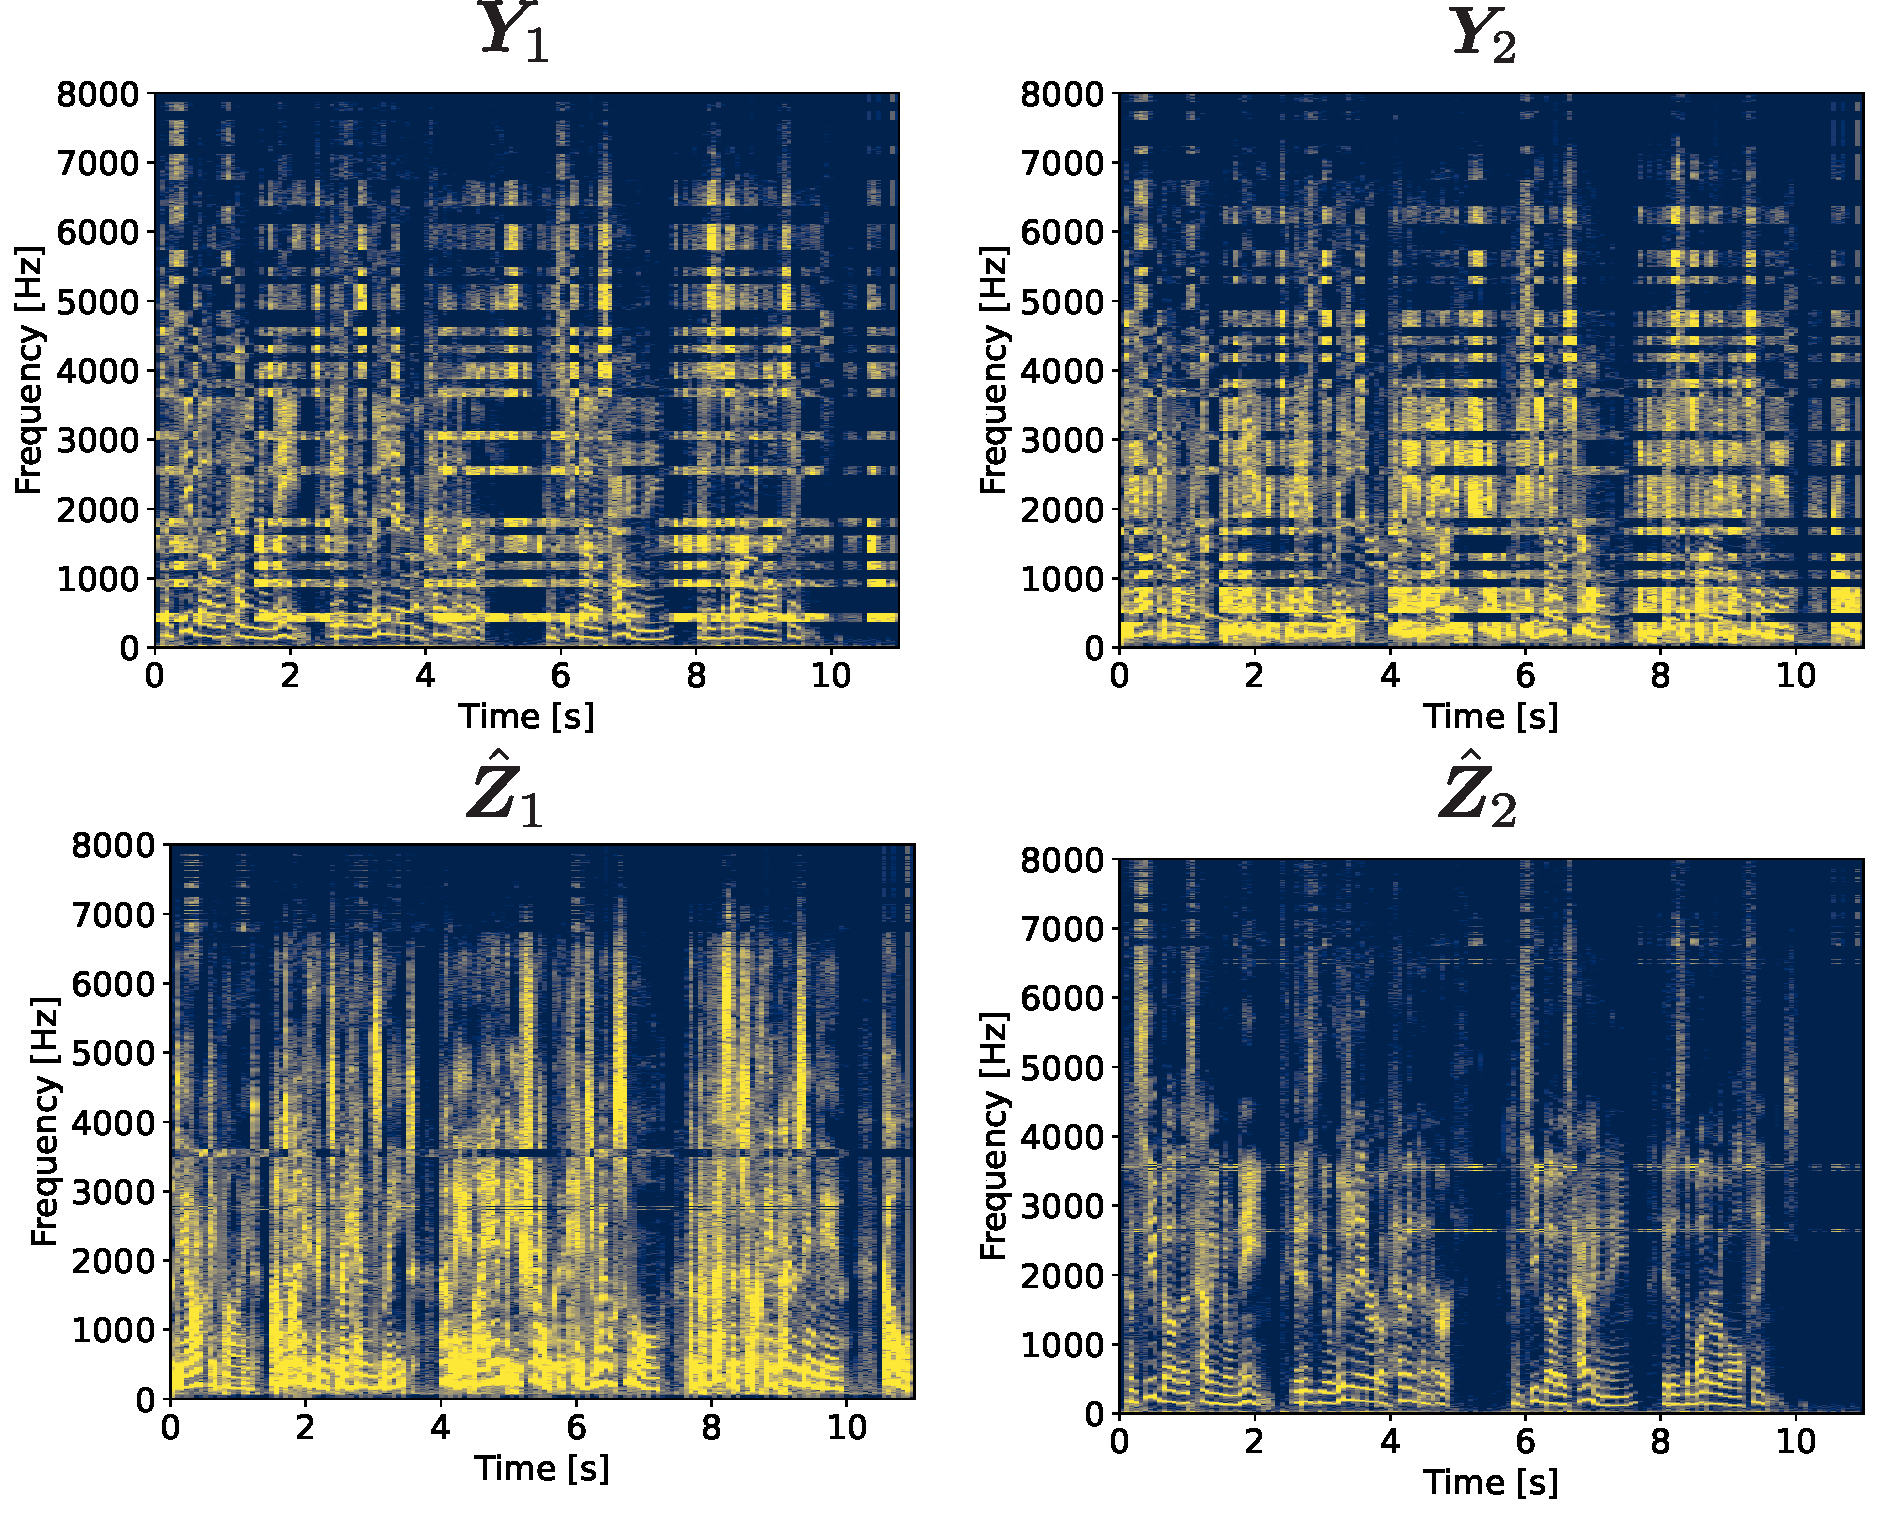
\includegraphics[clip, width=5.0in]{figures/audio_16block.pdf}
  \label{fig:spec_audio_16block}}
  \caption{Experimental results with $\gamma=16$ using speech source spectrograms of Fig.~\ref{fig:audio}. }
  \label{fig:audio_16block}
\end{figure*}
%%%%%%%%%%%%%%%%%%%%%%%%%%%%

%%%%%%%%%%%%%%%%%%%%%%%%%%%%
\begin{figure*}[!t]
  \centering
  \subfloat[Accuracy for training and validation data.]{\includegraphics[clip, width=4.5in]{figures/graph/Drum_16block.pdf}
  \vspace{-15pt}
  \label{fig:acc_Drum_16block}}
  \\
  \subfloat[Input spectrograms with permutation problem (upper) and permutation-aligned spectrograms using predicted results (bottom).]{\includegraphics[clip, width=5.0in]{figures/Drum_16block.pdf}
  \label{fig:spec_Drum_16block}}  
  \caption{Experimental results with $\gamma=16$ using musical instrument source spectrograms of Fig.~\ref{fig:drum}.}
  \label{fig:Drum_16block}
\end{figure*}
%%%%%%%%%%%%%%%%%%%%%%%%%%%%

Figs.~\ref{fig:audio_16block}及び\ref{fig:Drum_16block}にはそれぞれ,Figs.~\ref{fig:audio}及び\ref{fig:drum}の音声及び音楽信号に対して16行毎にランダムに入れ替える場合($\gamma=16$)の実験結果を示している.
前項の結果と同様に,学習時の学習データ及び検証データに対する正答率(各図における(a))と検証データの入力及び予測結果(各図における(b))をそれぞれ示している.
音声及び音楽信号のどちらに対しても,検証データに対する正答率が90\%を超えており,推定分離信号$(\hat{\bm{Z}}_1, \hat{\bm{Z}}_2)$も概ね正確な並び替えができていることが分かる.
SDRの改善量は,Fig.~\ref{fig:audio_16block}の$\hat{\bm{Z}}_1$が26.7~dB,$\hat{\bm{Z}}_2$が31.0~dBであった.
また,Fig.~\ref{fig:Drum_16block}の$\hat{\bm{Z}}_1$が22.6~dB,$\hat{\bm{Z}}_2$が27.6~dBであった.
Figs.~\ref{fig:audio_16block}及び\ref{fig:Drum_16block}を比較すると,音楽信号の実験結果の方が,音声信号の実験結果よりも検証データに対する正答率が高いことが分かる.
これは,本実験で使用した2種類の楽器音(ドラムとピアノ)が,男女の音声信号に比べて明確に異なる時間周波数構造を持っているためと推測できる.
ドラムの音は,Fig.~\ref{fig:drum}の$\bm{Z}_1$のスペクトログラムに示すように,全周波数成分に対して大きなパワーの成分を持っている.
一方で,ピアノの音はFig.~\ref{fig:drum}の$\bm{Z}_2$のスペクトログラムに示すように,基本周波数とその整数倍という調波構造を持っており,ドラムとは大きく異なる時間周波数構造となっていることが分かる.
このような時間周波数構造の違いにより,提案手法のDNNは音声信号よりも高精度に推定分離信号を予測することができたと考えられる.
以上の実験より,ある程度のサイズを持つ周波数帯域で生じるブロックパーミュテーション問題に対しては,実際の音声及び音楽信号でも,提案する深層パーミュテーション解決法が高精度に正しい分離信号成分の並び替えを予測できることが確認された.

\clearpage
%----------------------------------------------
\section{本章のまとめ}
\label{sec:matome}
%----------------------------------------------
本章では,提案手法の有効性を確認するため,人工的に作成したデータと実際の音声及び音楽信号を用意し実験を行った.
実験の結果より,人工データを用いたブロック単位でのパーミュテーション問題に対しては,どのような行列であっても100\%に近い確率で解決できることを示した.
実際の音声及び音楽信号に対しても,ブロック単位でランダムに入れ替えが行われている場合は90\%を超える正答率になることを示した.
SDRの改善量は,音声信号に対して28~dB程度,音楽信号に対しては25~dB程度であった.
次章では,本論文における総括とした結論を述べる.
